\documentclass[conference]{IEEEtran}
\IEEEoverridecommandlockouts
\usepackage{iftex}
\usepackage{amsmath,amssymb}
\ifXeTeX                                    % Tectonic / XeLaTeX: Times via TeX Gyre Termes
  \usepackage[varg]{newtxmath}
  \usepackage{fontspec}
  \setmainfont{texgyretermes}[Extension=.otf, UprightFont=*-regular, BoldFont=*-bold,
    ItalicFont=*-italic, BoldItalicFont=*-bolditalic]
\else                                       % pdfLaTeX
  \usepackage[T1]{fontenc}
  \usepackage{newtxtext,newtxmath}
\fi
\usepackage{graphicx}
\usepackage{booktabs}
\usepackage{multirow}
\usepackage{array}
\usepackage{siunitx}
\sisetup{detect-all}
\usepackage[hyphens]{url}
\usepackage[hidelinks]{hyperref}
\usepackage{cite}
\usepackage{xcolor}
\usepackage{balance}
\graphicspath{{figures/}}

% Small helpers used throughout the sections
\newcommand{\ci}[2]{\,[#1,\,#2]}          % confidence interval
\newcommand{\protR}{\textsc{R}}
\newcommand{\protB}{\textsc{B}}
\newcommand{\protA}{\textsc{A}}

\begin{document}

\title{Interpretable Classical Forgery Detection on CASIA~v2.0:\\
Exposing Format Shortcuts and Evaluating Under Leak-Controlled Protocols}

\author{\IEEEauthorblockN{Smit Patel (ID 2479966)}
\IEEEauthorblockA{EDS 6364 --- Digital Image Processing\\
Final project report}}

\maketitle

\begin{abstract}
CASIA~v2.0 is one of the most widely used benchmarks for image forgery detection, and error-level-analysis (ELA)
classifiers commonly report accuracies around 90\% on it. We show that the benchmark as released can be solved
without looking at image content: file metadata alone separates authentic from tampered images with 0.990
balanced accuracy (AUC 0.999), because most tampered images are uncompressed TIFF files while the authentic images
are JPEGs. We therefore evaluate under leak-controlled protocols that re-encode every image (B) or resample and then
re-encode it (R), and we measure every method against the shortcut features that survive each protocol. Our
detector is built from eight interpretable classical techniques covering point processing, histogram processing,
spatial filtering, frequency-domain analysis and edge/keypoint detection: ELA, local histograms, noise, JPEG
ghosts, DCT double quantisation, edge sharpness and two copy-move matchers. Their evidence is summarised by
within-image inconsistency statistics and fused by a random forest. On a frozen test set evaluated once, it reaches
AUC 0.805~[0.779,~0.831] under the strict protocol R, against 0.712 for the shortcut features. The calibrated
detector judges 52\% of images with 86\% accuracy, and learned map fusion localises tampered regions with pixel
F1~0.198 (0.308 under B). The detector transfers to the unseen MICC-F220 copy-move dataset (AUC 0.972; 11 forged scenes). An ELA +
ResNet-18 baseline reaches AUC 0.994 only on the leaking files, where shortcut features alone reach 1.000;
under R it reaches 0.770, and on MICC-F220 its AUC (0.53) is consistent with chance. The system is released with an interactive interface that explains
every verdict.
\end{abstract}

\begin{IEEEkeywords}
image forensics, forgery detection, copy-move, splicing, error level analysis, dataset bias, CASIA v2.0
\end{IEEEkeywords}

\section{Introduction}\label{sec:intro}

Photographs are routinely edited, and some edits are made to deceive: an object is copied to hide or duplicate
something (\emph{copy-move}), or a region from another photograph is pasted in (\emph{splicing}). Detecting such
forgeries, and showing \emph{where} the image was changed, matters for journalism, insurance-fraud review and the
integrity of scientific images~\cite{piva2013overview,verdoliva2020overview}. Classical image forensics addresses
this with signal-level cues that editing leaves behind: inconsistent JPEG compression
histories~\cite{krawetz2007ela,farid2009ghost,lin2009dq}, inconsistent noise~\cite{mahdian2009noise}, unnatural
edges, and duplicated content~\cite{fridrich2003copymove,amerini2011sift}. These cues are interpretable: each
produces a map that a human can inspect.

This project set out to build such a detector from the five technique families of a digital image processing
course (point processing, histogram processing, spatial filtering, frequency-domain filtering, and edge and corner
detection) and to evaluate it on CASIA~v2.0~\cite{dong2013casia}, a standard benchmark with 12,614 images and
ground-truth masks. The plan was to classify each image as authentic or tampered, to localise the tampered region,
and to compare the classical pipeline with a convolutional network trained on ELA images, a popular approach that
reports accuracies around 90\% on CASIA~v2.0~\cite{sudiatmika2019ela,ali2022recompress}.

Auditing the dataset changed the project. In CASIA~v2.0 as released, most tampered images are uncompressed TIFF
files, while the authentic images are JPEGs, most of them saved with the standard IJG quantisation tables that no
tampered JPEG uses (Section~\ref{sec:dataset}). A classifier that sees only the file's metadata separates the two
classes with 0.990 balanced accuracy (Section~\ref{sec:leakage}). Any method trained on the raw files, including
ELA, whose output depends directly on the compression history, can therefore score highly without detecting
tampering. This is a textbook case of data leakage~\cite{kaufman2012leakage} and shortcut
learning~\cite{geirhos2020shortcut}.

We therefore treat leak control as a first-class part of the evaluation. Every image is processed under an explicit
protocol: A (the files as released), B (every image re-encoded once as JPEG), or R (every image downscaled, then
re-encoded; our main protocol). Under each protocol we measure how far \emph{shortcut} features, meaning global
statistics that could reveal the class without any tampering evidence, can go. Forensic features must beat that
bar. Everything is designed within-image: each technique compares a region with the rest of the same image, rather
than comparing images with each other.

\textbf{Contributions.}
\begin{itemize}\setlength\itemsep{0pt}
\item A \emph{dataset audit} of CASIA~v2.0: corrected forgery types, re-matched and validated masks, and a
leakage-safe split that keeps source images, exact duplicates and verified near-duplicates together
(Sections~\ref{sec:dataset}--\ref{sec:leakage}).
\item A \emph{shortcut study} that quantifies the format leak and defines protocols that remove most of it
(Section~\ref{sec:leakage}).
\item Eight \emph{interpretable forensic modules} spanning all five DIP technique families, summarised by
within-image inconsistency statistics and tuned on validation data only (Sections~\ref{sec:method}--\ref{sec:params}).
\item A \emph{rigorous evaluation}:
  \begin{itemize}\setlength\itemsep{0pt}
  \item grouped nested cross-validation, added value over the shortcuts with paired bootstrap confidence intervals,
  and a calibrated detector that abstains when unsure (Section~\ref{sec:classification});
  \item learned localisation (Section~\ref{sec:localisation});
  \item a one-time evaluation on a frozen test set (Section~\ref{sec:test});
  \item robustness to post-processing, synthetic forgeries with exact masks, and a second dataset
  (Section~\ref{sec:robustness}).
  \end{itemize}
\item A pre-registered comparison with an \emph{ELA-CNN baseline} under the same controls, which reaches AUC 0.994 only
on the leaking files, where shortcut features alone reach 1.000 (Section~\ref{sec:cnn}).
\item An \emph{interactive system} that explains every verdict with evidence maps and per-image feature
attributions (Section~\ref{sec:system}).
\end{itemize}

Section~\ref{sec:related} reviews related work, and Section~\ref{sec:conclusion} discusses limitations and
concludes. Reproducibility details are in Appendix~\ref{app:repro}.

\section{Related Work}\label{sec:related}

\textbf{Compression-based cues.} Error level analysis re-saves an image as JPEG and inspects the per-pixel
difference; regions with a different compression history respond differently~\cite{krawetz2007ela}. JPEG ghosts
generalise this idea by re-saving at many qualities and looking for regions whose error is minimal at a different
quality from the rest of the image~\cite{farid2009ghost}. Double-quantisation analysis detects the periodic
pattern that a second JPEG compression leaves in the histograms of DCT coefficients; regions pasted in after the
first compression lack it~\cite{popescu2004stats,lin2009dq,bianchi2012dq}. All three cues measure compression
history. This is why they are powerful, and also why they are exposed to a dataset in which the two classes differ
in compression history for reasons unrelated to tampering.

\textbf{Noise and edges.} A region taken from another photograph often carries a different noise level. Noise
inconsistencies can be measured with local noise estimators~\cite{mahdian2009noise}; we use Immerk{\ae}r's fast
estimator~\cite{immerkaer1996noise}. Boundaries of pasted objects can be unnaturally sharp or feathered, which
edge detectors such as Canny's~\cite{canny1986} make measurable.

\textbf{Copy-move detection.} Block-based methods describe overlapping blocks, for example by their DCT
coefficients, sort them and look for many similar pairs sharing one shift~\cite{fridrich2003copymove}.
Keypoint-based methods match SIFT features~\cite{lowe2004sift} of an image against itself and verify the matches
geometrically with RANSAC~\cite{fischler1981ransac}, which makes them robust to rotation and
scaling~\cite{amerini2011sift}. Christlein et al.\ compared both families systematically~\cite{christlein2012eval}.
We implement one method of each family and add matching against the mirrored image, because some CASIA copies are
flipped.

\textbf{Learned detectors.} CNNs have been trained directly for splicing and copy-move
detection~\cite{rao2016cnn}. Constrained first layers suppress image content and expose manipulation
traces~\cite{bayar2016constrained}. Two-stream detectors combine RGB with noise residuals~\cite{zhou2018rgbn}, and
ManTra-Net treats localisation as local anomaly detection on learned manipulation-trace
features~\cite{wu2019mantra}. A simpler, widely used
recipe feeds ELA or recompression-difference images to a CNN, with reported accuracies around 90\% on
CASIA~v2.0~\cite{sudiatmika2019ela,ali2022recompress}. These models are trained and tested on the dataset's files
as released. Section~\ref{sec:cnn} shows that under that condition a network of this kind can reach a very high
score without detecting tampering.

\textbf{Datasets and evaluation pitfalls.} CASIA~v2.0~\cite{dong2013casia} is among the most used benchmarks.
Revised ground-truth masks for it have been published~\cite{pham2019casia}, which indicates known problems with
its annotations. Other benchmarks include COVERAGE, whose authentic images contain similar-but-genuine objects to
provoke false copy-move alarms~\cite{wen2016coverage}, and MICC-F220 for copy-move~\cite{amerini2011sift}. More
generally, a model can succeed by exploiting a shortcut that correlates with the label in the benchmark but not in
deployment~\cite{geirhos2020shortcut}. Information about the target that reaches the features through the data
collection process is a form of leakage~\cite{kaufman2012leakage}. Model selection on the evaluation data inflates
results unless it is nested~\cite{cawley2010nested}. Our evaluation is built around these three risks: format
shortcuts are controlled by protocols, near-duplicates are grouped in the split, and all selection is nested or
done on validation data, with a single evaluation of the frozen test set.

\section{The CASIA v2.0 Dataset and Its Pitfalls}\label{sec:dataset}

We use CASIA~v2.0~\cite{dong2013casia}, which has 12,614 images: 7,491 authentic and 5,123 tampered. The tampered
images were made with editing software as either \emph{copy-move} (a region duplicated within one image) or
\emph{splicing} (a region pasted from a different image). There are nine scene categories, and most images are
small: 85.8\% of authentic and 64.7\% of tampered images are $384\times256$ or $256\times384$ pixels.

\subsection{Labels and Masks}\label{sec:dataset-labels}

The forgery type is normally read from the file-name letter (Tp\_S = copy-move, Tp\_D = splicing), which gives
3,274 copy-move and 1,849 splicing images. For 115 images this letter conflicts with other evidence: the letter in
the mask's file name, and whether the host and donor ids are equal (equal ids mean copy-move). We take the majority
of these three votes, which changes 99 labels (60 splicing $\rightarrow$ copy-move, 39 copy-move $\rightarrow$
splicing). The corrected type (Table~\ref{tab:dataset-format}) is used for stratification and all per-type
results.

\begin{table}[t]
\centering
\caption{Class and file format (corrected forgery type)}\label{tab:dataset-format}
\footnotesize
\begin{tabular}{lrrrr}
\toprule
Class & Images & JPEG & TIFF & BMP \\
\midrule
Authentic & 7,491 & 7,437 & 0 & 54 \\
Copy-move & 3,295 & 967 & 2,328 & 0 \\
Splicing & 1,828 & 1,097 & 731 & 0 \\
\bottomrule
\end{tabular}
\end{table}

Each tampered image has a binary mask marking the content taken from the donor. Because 142 mask names differ
from their image name, we match masks on the trailing tamper id, which is unique across the dataset; every tampered
image then has exactly one mask. Of the 5,123 masks, 19 are unusable for pixel-level scoring (5 transposed, 12
with other sizes, 2 covering more than 95\% of the image). These images remain in the classification experiments
but are excluded from localisation scoring, which leaves 5,104 valid masks. Checked against where the tampered image
differs from its background image, the 5,034 checkable masks have median recall 0.885 and median precision 0.991,
so the masks are generally accurate; 52 masks with recall $<0.2$ are flagged but not removed.

Tampered regions are small: the median tampered area is 3.1\% of the image (10th percentile 0.5\%, 90th
percentile 28\%). We therefore report localisation in three area buckets: $<1\%$ (1,114 images), 1--5\%
(2,023) and $>5\%$ (1,967). A tampered file name names two authentic images; we treat the first-named one as the
\emph{host}, since it supplies most pixels in 1,689 of the 1,778 splicing-named images with differing ids. In 23
images the second-named image supplies most pixels (18 large pastes and 5 apparently swapped ids); these are
additionally grouped with the second-named image (Section~\ref{sec:leakage}). Details of the mask audit and the
host analysis are in Appendix~\ref{app:dataset}.

\subsection{Pitfalls That Affect Evaluation}\label{sec:dataset-pitfalls}

\emph{(1) File format tracks the label.} 60\% of tampered images are uncompressed TIFF, but no authentic image is
(Table~\ref{tab:dataset-format}). \emph{(2) JPEG settings track the label.} Among JPEG files, 89.1\% of authentic
images use a standard libjpeg (IJG) quantisation table, compared with 0\% of tampered images, whose tables look like
those written by editing software. The closest IJG quality factor is mostly 84 or 90 for authentic images and 93
for tampered ones. \emph{(3) Image size tracks the label.} Tampered images are more often $640\times480$ or
$800\times600$. \emph{(4) Duplicates.} 196 authentic images appear twice under different ids with identical
pixels, and about 480 tampered images are near-identical to an authentic image other than their named host.
\emph{(5) Label noise in names}, corrected as described above.

Points 1--3 mean that a classifier can separate the classes without looking at any forensic evidence.
Section~\ref{sec:leakage} measures this directly.

\section{Leakage-Safe Splits, Protocols and the Shortcut Study}\label{sec:leakage}

\subsection{Leakage-Safe Splits}\label{sec:leakage-splits}

A tampered image shares most of its pixels with its host image. If the host is in the training set and the tampered
version in the test set, the evaluation is optimistic. We therefore split by \emph{groups}, built with union-find
over four kinds of link: the host id; exact pixel duplicates (196 merges); verified near duplicates (17 merges from
694 pairs); and the second-named id, for the 23 images where that image supplies most of the pixels (16 merges).
The result is 7,262 split groups of at most 69 images (near-duplicate criteria in Appendix~\ref{app:leakage}).

Stratified group $k$-fold assignment (20 bins, seed 42) with strata of forgery type $\times$ file format gives
train 8,828 / val 1,894 / test 1,892 images (70.0/15.0/15.0\%). The train+val (``dev'') set is further
divided into five grouped CV folds. No group crosses a split or a fold; this is asserted before the split is
written and checked again by the test suite. The split is frozen by SHA-256 hashes; it was re-frozen once, before
any model had seen the test set, after the forgery-type labels were corrected and the donor-dominant links added.
The test set stays unused until the final evaluation (Section~\ref{sec:test}).

One limitation remains. For 830 tampered images (828 splicing), the donor image is in a different split. The shared
content is the pasted region: a median of 5.5\% of the image, and 34.5\% at the 90th percentile. We report this
rather than prevent it: merging every donor would create a single group of 4,027 images (31.9\% of the dataset),
which makes a stratified 70/15/15 split impossible.

\subsection{Evaluation Protocols}\label{sec:leakage-protocols}

\emph{A (as released):} images exactly as distributed. \emph{C (JPEG-only):} A restricted to JPEG files of both
classes, an intuitive way to remove the format cue. \emph{B (re-encoded, Q=85):} every image is decoded and re-encoded
once to JPEG at quality 85 with 4:2:0 chroma subsampling, so all images share one container format and one
quantisation table. \emph{R (resampled + re-encoded, ``strict''):} every image is downscaled by 0.75 with area
interpolation, then re-encoded as in B; masks are resized with nearest-neighbour interpolation.

\subsection{Shortcut Study}\label{sec:leakage-shortcuts}

We train a random forest~\cite{breiman2001rf} (300 trees, balanced class weights) on feature families computed
\emph{globally over the whole image}, none of which localises anything: \emph{file metadata} (format flags,
quantisation-table statistics); \emph{image dimensions}; \emph{naive global ELA} (statistics of one ELA residual at
Q=90); and \emph{compression history} (global double-quantisation histograms of low-frequency DCT coefficients and
a global JPEG-ghost curve). Table~\ref{tab:leakage} and Fig.~\ref{fig:leakage} give balanced accuracy on the five
grouped dev folds (chance is 0.5); the full feature lists and ROC-AUCs are in Appendix~\ref{app:leakage}.

\begin{table}[t]
\centering
\caption{Global shortcut features alone: balanced accuracy (5-fold grouped CV on dev) per protocol}\label{tab:leakage}
\footnotesize
\begin{tabular}{lcccc}
\toprule
Features & A & C & B & R \\
\midrule
File metadata & \textbf{0.990} & \textbf{0.991} & 0.508 & 0.503 \\
Image dimensions & 0.603 & 0.597 & 0.603 & 0.604 \\
Naive global ELA & 0.696 & 0.678 & 0.564 & 0.539 \\
Compression history & 0.928 & 0.955 & \textbf{0.789} & 0.608 \\
All shortcuts & 0.989 & 0.986 & \textbf{0.797} & \textbf{0.649} \\
\bottomrule
\end{tabular}
\end{table}

\begin{figure*}[t]
\centering
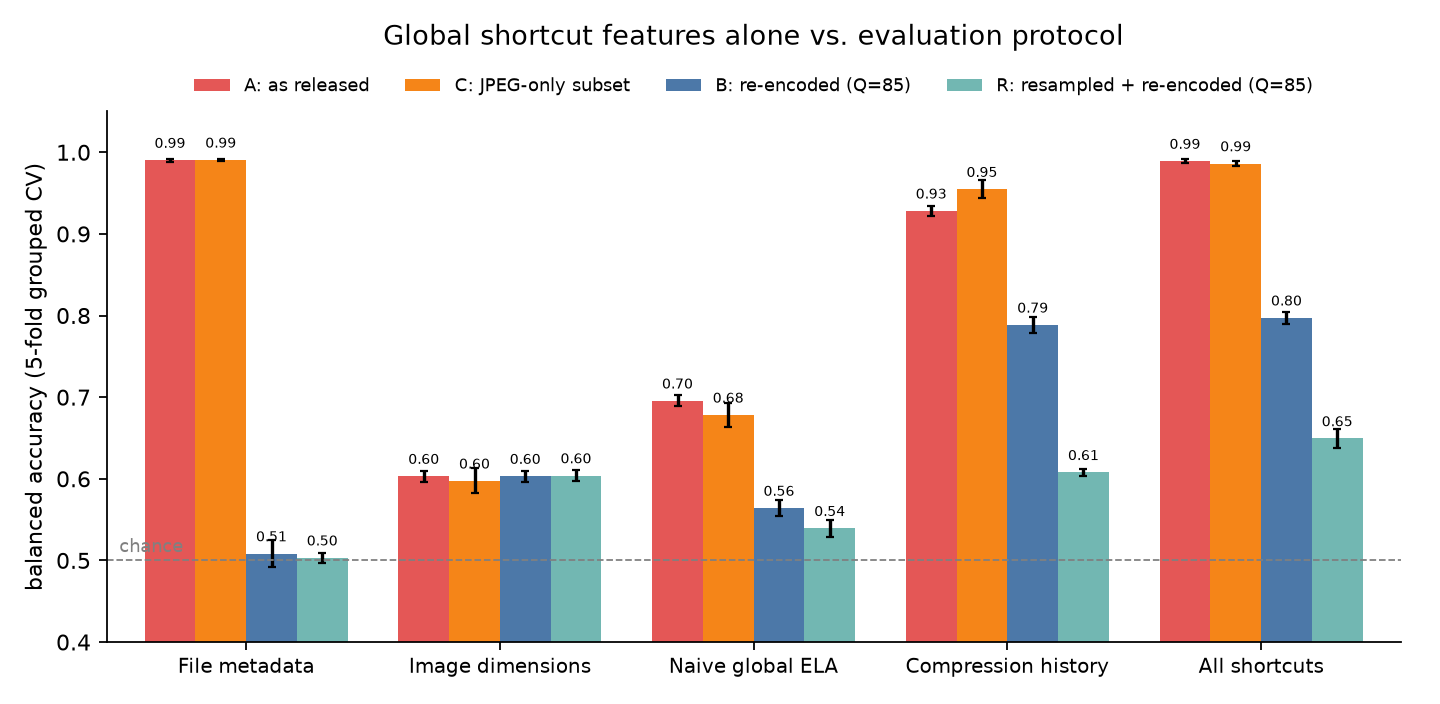
\includegraphics[width=0.82\textwidth]{fig_leakage.png}
\caption{Balanced accuracy (mean and standard deviation over the five grouped dev folds) of a random forest trained
only on global shortcut features, under protocols A, C, B and R. The dashed line marks chance (0.5).}
\label{fig:leakage}
\end{figure*}

\textbf{The benchmark as released can be solved almost perfectly without looking at image content.} File metadata
alone reaches 99.0\% balanced accuracy (AUC 0.999). \textbf{Restricting to JPEG files does not fix this}: the
quantisation tables still separate the classes (99.1\%). \textbf{Re-encoding (B) removes the container/metadata
shortcut (0.508) but not the compression history.} A global double-quantisation and ghost-curve classifier still
reaches 0.789 under B. Each image carries its earlier compression history: authentic images were last saved as
JPEGs with standard libjpeg tables (89\% of them), while tampered images were last saved as editing-software JPEGs
or as uncompressed TIFFs, and one extra re-encode does not erase that history. The effect is strongest when both
classes started as JPEG: 0.919 on JPEG sources alone, against 0.725 for authentic vs.\ TIFF-tampered.
\textbf{Resampling before re-encoding (R) erases most of it.} Compression history falls to 0.608, and all shortcuts
together reach 0.649 $\pm$ 0.011; most of what remains is the image-size shortcut. \textbf{Image size is a residual
shortcut (0.60) that no protocol removes}, so the forensic pipeline must never use raw image dimensions as
features. Finally, \textbf{naive global ELA is weak once the container is controlled} (0.56 under B). Even under A
it reaches only 0.70, and it gains nothing from TIFF files: it scores 0.68 under C, where no TIFFs remain. Its
signal is compression history, not tampering.

% Module table (Section V) placed here so that the full-width float appears next to Section V.
\begin{table*}[t]
\centering
\caption{The eight forensic modules, the DIP technique family each one uses, and the evidence it computes}\label{tab:modules}
\scriptsize
\begin{tabular}{@{}c >{\raggedright\arraybackslash}p{2.3cm} >{\raggedright\arraybackslash}p{1.9cm} >{\raggedright\arraybackslash}p{8.6cm} >{\raggedright\arraybackslash}p{2.4cm}@{}}
\toprule
\# & Module & DIP category & Evidence & Main parameters \\
\midrule
1 & Error Level Analysis & Point processing &
$|I - \mathrm{JPEG}_q(I)|$ averaged per $8\times8$ block, divided by (block texture $+\,c$) so busy regions are not
mistaken for tampering & $q$, block, $c$ \\
2 & Patch-histogram $\chi^2$ & Histogram processing &
ELA residual contrast-stretched and histogram-equalised; $\chi^2$ distance of each patch histogram to the image's
reference histogram (the mean over textured patches) & $q$, patch, bins \\
3 & Noise level & Spatial filtering &
Immerk{\ae}r high-pass kernel (or a $3\times3$ Laplacian); per-block robust $\sigma = 1.4826\cdot\mathrm{median}|r|$
over non-edge pixels (gradient $\leq$ a global quantile), since edges leak content into the residual; flat and
clipped blocks excluded via the common validity mask & kernel, block, edge quantile \\
4 & JPEG ghosts & Point processing &
Per-block squared re-compression error at Q = 50 \ldots 95; each block's curve is min-max normalised; evidence =
L1 distance from the image's median curve & block \\
5 & DCT double quantisation & Frequency domain &
Per $8\times8$ DCT frequency: last quantisation step (known or estimated), test of the coefficient histogram for
periodicity, and per-coefficient posterior of \emph{not} following the periodic pattern; block log-odds averaged
over frequencies & number of frequencies, period threshold \\
6 & Edge sharpness & Edge detection &
Canny edges; at each edge pixel, sharpness = gradient / local contrast ($5\times5$ max $-$ min); block median; both
over-sharp (hard cut-out) and over-soft (feathered) outliers count & Canny thresholds, block \\
7 & Copy-move: keypoints & Corner/keypoint detection &
SIFT (or Harris) keypoints with SIFT descriptors; g2NN matching of the image against itself and against its mirror
image; pairs $<20$\,px apart dropped; RANSAC affine fit, separately for direct and mirrored matches & detector,
ratio, contrast \\
8 & Copy-move: blocks & Frequency domain &
Overlapping $16\times16$ blocks described by 9 low-frequency DCT coefficients; the blocks of the image and of its
mirror are sorted lexicographically together; near-identical neighbours are paired and their shift vectors voted on
& tolerance, min.\ block std, min.\ votes \\
\bottomrule
\end{tabular}
\end{table*}

\subsection{Consequences for the Rest of the Project}\label{sec:leakage-consequences}

A forensic feature set shows real tampering evidence only if it clearly beats the shortcuts under the same
protocol: 0.797 $\pm$ 0.007 balanced accuracy (AUC 0.876) under B and 0.649 (AUC 0.720) under R. These are lower
bounds; a stronger global probe might score higher. We therefore report classification under both B and R,
measure the \emph{added value} of the forensic features over the shortcuts, and choose the main protocol with a
rule fixed before the classification results were seen (Section~\ref{sec:classification}). Pixel-level
localisation cannot be gamed by global shortcuts, so we treat it as the most trustworthy result, and the features
favour \emph{within-image inconsistency} over absolute global statistics (Section~\ref{sec:method}). For B we keep
Q=85, which suppresses the shortcuts about as well as Q=75 while discarding less image detail
(Appendix~\ref{app:leakage}).

\section{Method: Forensic Feature Modules}\label{sec:method}

\subsection{Common Design}\label{sec:method-design}

Every module maps an RGB image to two outputs: an \emph{evidence map} (float, $[0,1]$, image-sized; bright =
suspicious), used for localisation, and a set of \emph{scalar features}, used for image-level classification.
Section~\ref{sec:leakage} showed that \emph{global} image statistics on CASIA~v2.0 largely measure compression
history rather than tampering. Each module therefore reduces its evidence to a \emph{block map} and describes it
with \emph{within-image inconsistency} statistics (\texttt{local\_*}). All of these are scale-free, so they compare
a region with the rest of the same image rather than with other images: the robust z-score of the most extreme
block and its 99th percentile, where $z = (\text{value} - \text{median}) / (1.4826\cdot\text{MAD})$; the share of
blocks with $z>3$; the size of the largest connected cluster of blocks with $z>2.5$; Moran's~$I$ spatial
autocorrelation~\cite{moran1950}; and the mean robust z-score of the top 5\% of blocks, which stays scale-free for
signed and log-valued maps. Absolute image-wide levels are kept separately as \texttt{global\_*} features, so that
Section~\ref{sec:classification} can test whether they act as shortcuts.

\emph{Flat and clipped regions carry no evidence.} A textured object on a plain black background has, trivially, a
different error level and noise level from its surroundings. Blocks whose grey-level standard deviation is below a
threshold, or whose mean is within 4 grey levels of black or white, are therefore excluded from the statistics and
receive zero evidence. This was added after a sanity check showed four modules lighting up on an authentic studio
photograph. All modules, including the noise module, use the same validity mask.

\subsection{The Eight Modules}\label{sec:method-modules}

Table~\ref{tab:modules} lists the modules and the DIP technique family each one exercises. Together they cover all
five families required by the course: \emph{point processing} (ELA~\cite{krawetz2007ela} and JPEG
ghosts~\cite{farid2009ghost}), \emph{histogram processing} (patch-histogram $\chi^2$ on a histogram-equalised
residual), \emph{spatial filtering} (the Immerk{\ae}r noise residual~\cite{immerkaer1996noise}), the
\emph{frequency domain} (DCT double quantisation after Lin et al.~\cite{lin2009dq}, and block-DCT copy-move
matching~\cite{fridrich2003copymove}), and \emph{edge and corner detection} (Canny~\cite{canny1986} edge
sharpness, and SIFT~\cite{lowe2004sift} or Harris~\cite{harris1988} keypoints for copy-move detection with g2NN
matching~\cite{amerini2011sift} and RANSAC~\cite{fischler1981ransac}). Fig.~\ref{fig:modules} shows the evidence
maps of all eight modules under protocol R.

\begin{figure*}[t]
\centering
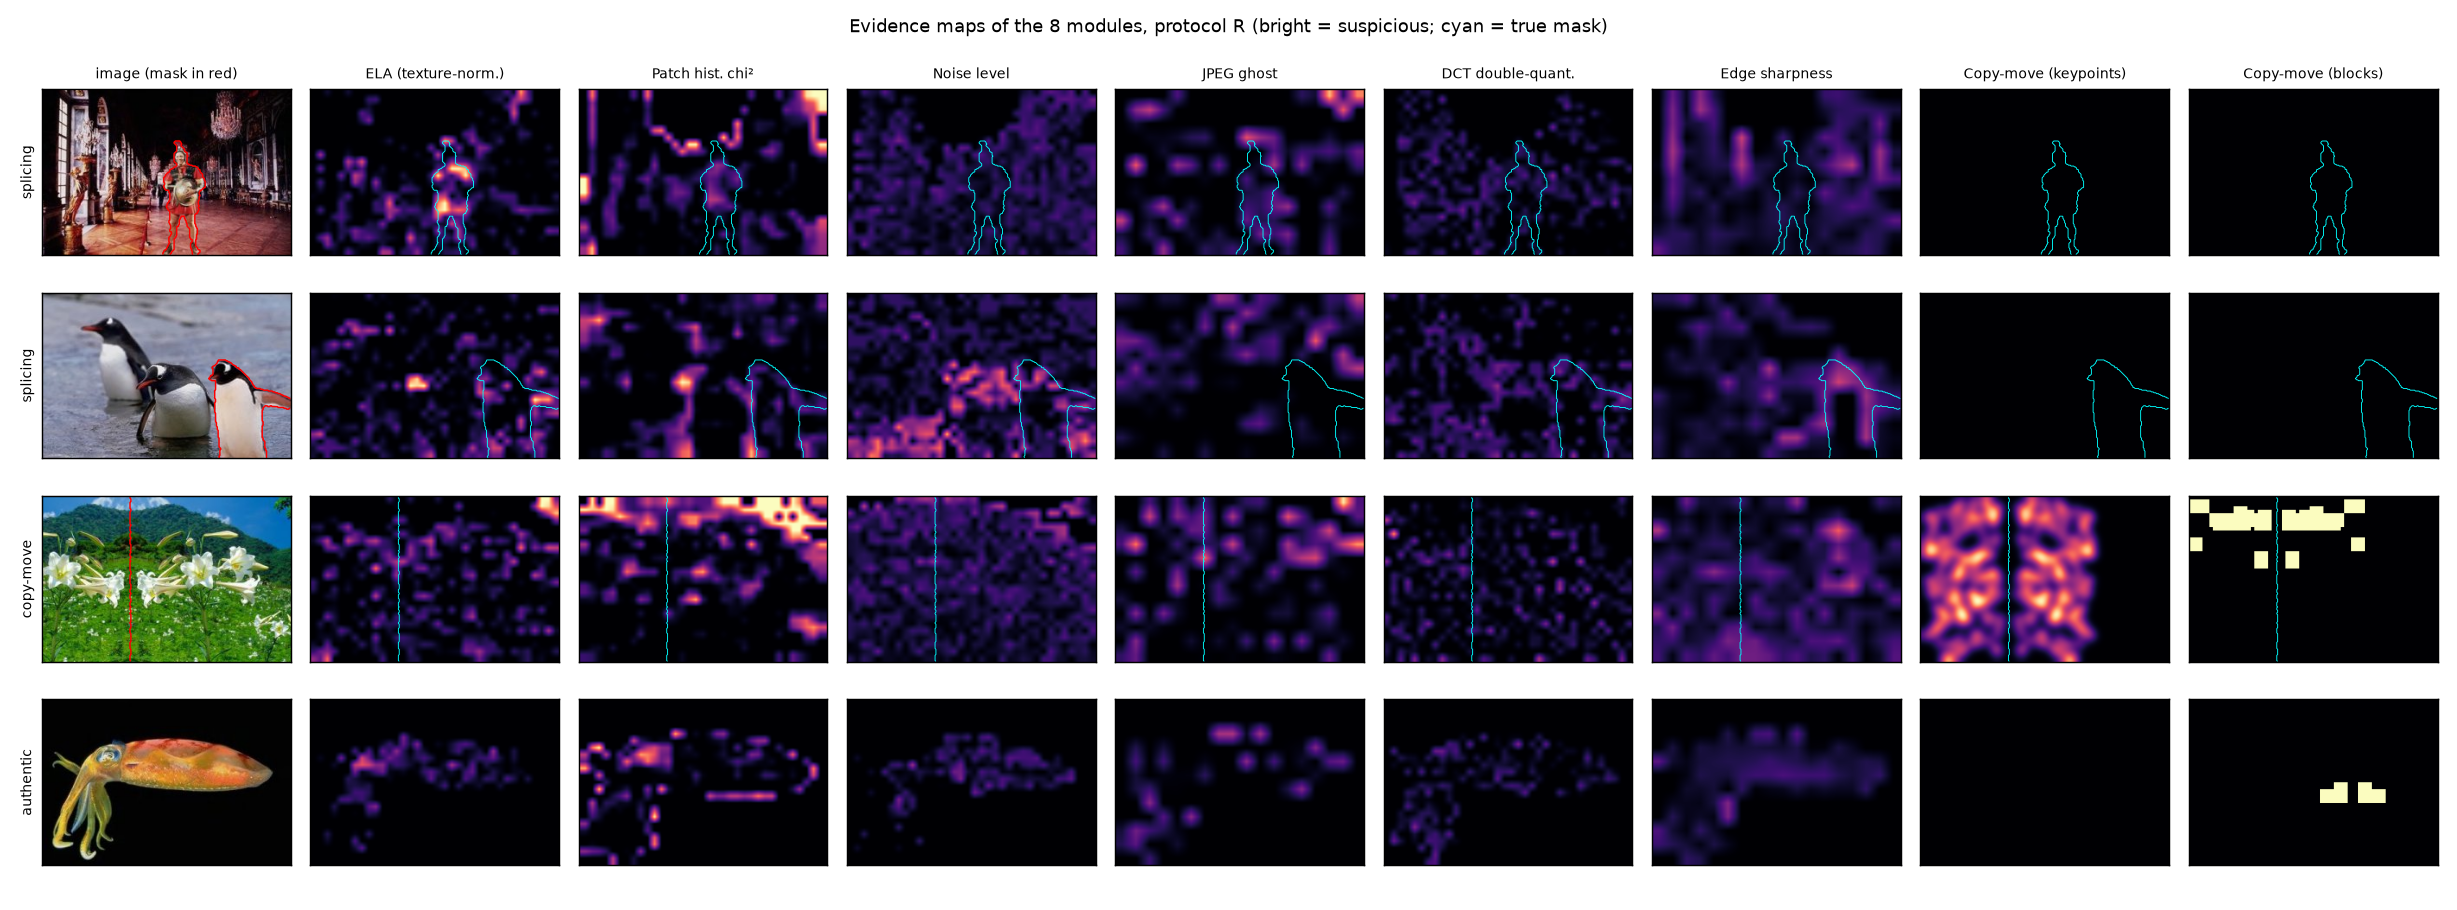
\includegraphics[width=\textwidth]{fig_modules_R.png}
\caption{Evidence maps of the eight modules under protocol R (bright = suspicious) for two splicing images, one
copy-move image and one authentic image. The first column shows the image with its ground-truth mask in red; the
other columns outline the mask in cyan.}
\label{fig:modules}
\end{figure*}

\subsection{DCT and Copy-Move Details}\label{sec:method-details}

Under B and R the DCT module uses the exact IJG Q85 quantisation table (a blind step estimate is used only when
the last compression is unknown) and declares a frequency periodic when a permutation test on its detrended
log-histogram gives $p\leq\alpha$, with $\alpha$ tuned in Section~\ref{sec:params}; on dedicated test
cases at $\alpha=0.01$ the false-positive rate is 0--3\%, against 16--48\% for an earlier fixed threshold, but some regular
double-quantisation patterns are missed (Appendix~\ref{app:method}). Because several CASIA copy-moves are
horizontally flipped, both copy-move detectors also match the image against its mirror image, and keypoint pairs
are oriented left-to-right before RANSAC; one RANSAC fit is run per matching mode (direct and mirrored), so the
keypoint detector recovers at most one copied region per mode.

\subsection{Verification}\label{sec:method-verification}

Each module has a unit test on a \emph{synthetic forgery with a known region} (e.g.\ an uncompressed region
inside a Q60 image for ELA, a single-compressed region inside a double-compressed image for DCT, plain and mirrored
copies for copy-move; full list in Appendix~\ref{app:method}). In every case the evidence map is clearly higher
inside the planted region, and a clean image yields no copy-move votes. Contract tests cover tiny, narrow, flat and
black images, and check determinism.

\section{Parameter Selection}\label{sec:params}

Parameters were tuned on training and validation images only; the test set is untouched. A fixed random sample of
2,400 training images (1,200 authentic, 1,200 tampered) is used for fitting and 1,000 validation images (500 / 500)
for scoring. These 3,400 dev images later appear in the cross-validation folds of
Section~\ref{sec:classification}, so those AUCs are not fully independent of this tuning, a source of mild
optimism. Each module is tuned on its own by coordinate ascent (one parameter at a time, the others held at their
current best), always from the same defaults, so a re-run reproduces the same choices. A setting is scored
by the mean of two numbers: the \emph{image AUC} of a random forest trained on the module's \texttt{local\_*}
features only, so global shortcuts cannot inflate the score; and the \emph{pixel AUC}, the mean pixel-level ROC-AUC
of the evidence map against the ground-truth mask over the validation tampered images (copy-move images only for
the two copy-move modules). A new value is adopted only if it improves the score by more than 0.002. Parameters are
chosen under protocol B and reused unchanged under R. After corrections to the DCT, noise and both copy-move
modules, all eight modules were re-tuned from their defaults with the final code. Table~\ref{tab:params} gives the
resulting scores; the chosen values and the sweep curves are in Appendix~\ref{app:params}
(Table~\ref{tab:params-chosen}, Fig.~\ref{fig:sweeps}).

\begin{table}[t]
\centering
\caption{Validation scores of each module with its chosen parameters (image AUC from \texttt{local\_*} features
only; share = images with pixel AUC $>0.6$ under B)}\label{tab:params}
\footnotesize
\begin{tabular}{@{}lccccc@{}}
\toprule
 & \multicolumn{2}{c}{Image AUC} & \multicolumn{2}{c}{Pixel AUC} & \\
\cmidrule(lr){2-3}\cmidrule(lr){4-5}
Module & B & R & B & R & Share \\
\midrule
ELA & 0.696 & 0.638 & 0.615 & 0.625 & 0.52 \\
Patch hist.\ $\chi^2$ & 0.571 & 0.511 & 0.589 & 0.563 & 0.44 \\
Noise level & 0.609 & 0.592 & 0.560 & 0.544 & 0.41 \\
JPEG ghosts & 0.745 & 0.602 & 0.645 & 0.542 & 0.58 \\
DCT double quant. & 0.797 & 0.491 & 0.668 & 0.543 & 0.65 \\
Edge sharpness & 0.610 & 0.575 & 0.574 & 0.568 & 0.46 \\
Copy-move keypoints & 0.744 & 0.728 & 0.719 & 0.683 & 0.56 \\
Copy-move blocks & 0.618 & 0.561 & 0.527 & 0.517 & 0.14 \\
\bottomrule
\end{tabular}
\end{table}

\textbf{The sweeps mainly improved localisation.} The largest pixel-AUC gains over the defaults were ELA
(0.551 $\rightarrow$ 0.615), noise (0.491 $\rightarrow$ 0.560) and DCT double quantisation (0.630 $\rightarrow$
0.668). For ELA, the lower re-save quality ($q=85$) had the largest effect (0.551 $\rightarrow$ 0.613). The gains
were not uniform: because the criterion is the mean of both scores, a gain in one can offset a small loss in the
other (e.g.\ for the noise and edge modules).

\textbf{Harris corners, proposed originally, are not a usable copy-move detector on these images.} On CASIA's small
($384\times256$) images they yield few, poorly repeatable points: image AUC 0.564 and pixel AUC 0.512, against 0.744
and 0.719 with SIFT's scale-invariant detector. We therefore use SIFT and report Harris as a negative result.
\textbf{Block matching localises few copy-moves} (pixel AUC $>0.6$ for 14\% of images, against 56\% for
keypoints), presumably because many CASIA copy-moves involve geometric transformations (not measured) and block DCT
features are not invariant to rotation or scale.

\textbf{Protocol R removes what the compression modules rely on.} DCT double quantisation falls from 0.797 to 0.491
image AUC and from 0.668 to 0.543 pixel AUC, and JPEG ghosts from 0.745 to 0.602 image AUC; resampling breaks the
$8\times8$ JPEG grid, so this is expected. Modules that do not depend on the grid are much less affected: copy-move
keypoints 0.744 $\rightarrow$ 0.728, ELA 0.696 $\rightarrow$ 0.638, edges 0.610 $\rightarrow$ 0.575. These
localisation scores come from inconsistency within each image, so global shortcuts cannot produce them. Under B,
the DCT and ghost modules localise pasted regions (pixel AUC 0.67 and 0.65): the pasted content has a different
compression history \emph{from the rest of the same image}, which is genuine tampering evidence. The choice between
B and R as the main protocol is made in Section~\ref{sec:classification}.

\section{Image-Level Classification}\label{sec:classification}

\subsection{Set-up}\label{sec:classification-setup}
All 10,722 development images (train + val) are used with the five grouped folds of Section~\ref{sec:leakage}; the test set is untouched (Section~\ref{sec:test}). Two classifiers are compared: an RBF SVM \cite{cortes1995svm} on standardised features ($C \in \{1, 10, 100\}$, $\gamma \in \{0.3, 1, 3\}/d$) and a random forest (RF) \cite{breiman2001rf} with 300 trees and balanced class weights (max features $\in \{\sqrt{d}, 0.3d\}$, min leaf $\in \{1, 4\}$), both from scikit-learn \cite{pedregosa2011sklearn}. Hyper-parameters are selected inside each training fold by grouped 3-fold CV maximising ROC-AUC, i.e.\ nested CV \cite{cawley2010nested}. We report mean $\pm$ std over the five folds and the pooled out-of-fold AUC with a 95\% CI from 1,000 group-bootstrap resamples \cite{efron1993bootstrap}, in which split groups are resampled whole. Four feature sets are fused: \emph{forensic, local only} (the 70 within-image inconsistency features), \emph{forensic, local + global} (82 features), \emph{shortcuts} (the 49 global features of Section~\ref{sec:leakage}) and \emph{forensic + shortcuts}.

A main-protocol rule was fixed before the results were seen: the main protocol is R if, under R, adding the forensic features to the shortcuts raises AUC with a 95\% CI excluding 0; otherwise B under the same test; otherwise none. The outcome is R.

\begin{table}[!t]
\centering
\caption{Out-of-fold ROC-AUC (mean over 5 folds; standard deviations in Appendix~\ref{app:classification}). Protocol A exists only to show the leak.}
\label{tab:cls-auc}
\footnotesize
\setlength{\tabcolsep}{4pt}
\begin{tabular}{lccccc}
\toprule
Features & B: RF & B: SVM & R: RF & R: SVM & A: RF \\
\midrule
Shortcuts & 0.876 & 0.876 & 0.721 & 0.771 & \textbf{1.000} \\
Forensic, local & 0.902 & -- & \textbf{0.781} & -- & 0.962 \\
Forensic, loc.+glob. & 0.910 & 0.892 & \textbf{0.795} & 0.793 & 0.978 \\
Forensic + shortcuts & 0.926 & 0.922 & 0.810 & \textbf{0.826} & 0.999 \\
\bottomrule
\end{tabular}
\end{table}

\begin{table}[!t]
\centering
\caption{Added value over the shortcuts: paired group-bootstrap $\Delta$AUC [95\% CI].}
\label{tab:cls-added}
\footnotesize
\setlength{\tabcolsep}{4pt}
\begin{tabular}{lcc}
\toprule
 & (Forensic + shortcuts) & Forensic (local only) \\
 & $-$ shortcuts & $-$ shortcuts \\
\midrule
B: RF & +0.050\ci{0.044}{0.055} & +0.026\ci{0.018}{0.033} \\
R: RF & \textbf{+0.088}\ci{0.078}{0.097} & \textbf{+0.059}\ci{0.047}{0.072} \\
R: SVM & +0.054\ci{0.045}{0.063} & -- \\
A: RF & $-$0.000 & $-$0.037 \\
\bottomrule
\end{tabular}
\end{table}

\subsection{Results}\label{sec:classification-results}
Table~\ref{tab:cls-auc} gives the out-of-fold AUCs and Table~\ref{tab:cls-added} the added value over the shortcuts. Under R, the forensic RF (local + global) reaches AUC 0.795\ci{0.783}{0.806}, and, at threshold 0.5 on the uncalibrated forest, balanced accuracy 0.705~$\pm$~0.011 and image-level F1 0.628~$\pm$~0.018 (not the pixel F1 of Section~\ref{sec:localisation}). Three findings stand out. First, \emph{the forensic features carry real tampering evidence}: under both honest protocols they beat every shortcut combined and add significantly on top of them. The purest test is the local-only set, which compares regions within one image; it beats the shortcuts by +0.059 AUC under R and +0.026 under B, both with CIs well above zero. Second, \emph{on the dataset as released (A) the numbers are meaningless}: shortcuts alone score AUC 1.000 and adding the forensic features changes nothing ($\Delta$AUC $-$0.000). An A-protocol forensic AUC of 0.978 would look state-of-the-art, but most of it is compression history. Third, \emph{RF and SVM are statistically indistinguishable} on the forensic features under R (McNemar test \cite{mcnemar1947}: 603 vs 644 discordant decisions, $p = 0.26$); the SVM combines forensic and shortcut features somewhat better (0.826 vs 0.810).

\emph{Ablations} (RF, fixed hyper-parameters; Appendix~\ref{app:classification}). Under B the compression modules lead when used alone (DCT 0.821, ghosts 0.758); resampling (R) removes their signal, as Section~\ref{sec:params} predicted. Copy-move keypoint matching is the most robust module (0.747 $\to$ 0.720 from B to R) and the most important one under R: removing it costs 0.080 AUC (under B, 0.039, just behind DCT at 0.046). Under R, ELA is the second pillar (0.013). Removing the noise, histogram or block-matching module changes AUC by 0.004 or less; their information is redundant with ELA and the keypoint detector, and they are kept for completeness and localisation.

\begin{table}[!t]
\centering
\caption{Where the detector succeeds and fails (R, RF, out-of-fold). Detection rate at threshold 0.5.}
\label{tab:cls-breakdown}
\footnotesize
\begin{tabular}{lcc}
\toprule
Subset & Detection rate & AUC \\
\midrule
Copy-move vs authentic & -- & 0.851 \\
Splicing vs authentic & -- & 0.694 \\
Tampered area $<$ 1\% & 0.525 & 0.768 \\
Tampered area 1--5\% & 0.530 & 0.787 \\
Tampered area $>$ 5\% & 0.596 & 0.818 \\
Tampered, released as TIFF & 0.606 & -- \\
Tampered, released as JPEG & 0.477 & -- \\
\midrule
Authentic (false-positive rate) & 14.4\% & -- \\
\bottomrule
\end{tabular}
\end{table}

\emph{Per forgery type and error breakdown} (Table~\ref{tab:cls-breakdown}). Copy-move is detected far better than splicing (AUC 0.851 vs 0.694): copy-move leaves an explicit duplicate, whereas splicing must be found through subtler statistical differences. Larger regions are easier, as expected; the 16 tampered images without a valid mask are in no area bucket. Tampered images released as TIFF are detected more often than JPEG ones even under R, so some format-related difference may survive resampling; this residual bias is re-checked on the test set (Section~\ref{sec:test}). A second forest, trained on tampered images only, predicts copy-move vs splicing with out-of-fold AUC 0.830 (R) / 0.874 (B) and supplies the ``likely type'' output.

\subsection{Calibration and the ``Uncertain'' Verdict}\label{sec:classification-calib}
The raw forest is already fairly well calibrated under R: its expected calibration error (ECE, the sample-weighted mean gap between predicted and observed tampered share over 10 equal-width probability bins) is 0.034, and isotonic calibration \cite{zadrozny2002calib}, fitted inside each fold, brings it to 0.009 (Brier 0.176 $\to$ 0.175; Fig.~\ref{fig:calibration} in Appendix~\ref{app:classification}). Accuracy on the images the system is willing to judge rises steadily as the uncertain band widens: 0.731 when judging every image, 0.855 at 51\% coverage and 0.959 at 12\% coverage. The band is the smallest that reaches 85\% accuracy while still judging at least half of the images. Under R this gives $P(\text{tampered}) \in 0.5 \pm 0.24$, judging 51\% of images with accuracy 0.855 (balanced accuracy 0.810); under B, $0.5 \pm 0.04$, judging 96\% with accuracy 0.851 (balanced 0.839). The 85\% target is plain accuracy on an imbalanced dev set (59\% authentic), hence the balanced accuracies. Under the strict protocol R the tool honestly declines to judge about 49\% of CASIA images; this is the cost of refusing the shortcuts.

\begin{figure*}[!t]
\centering
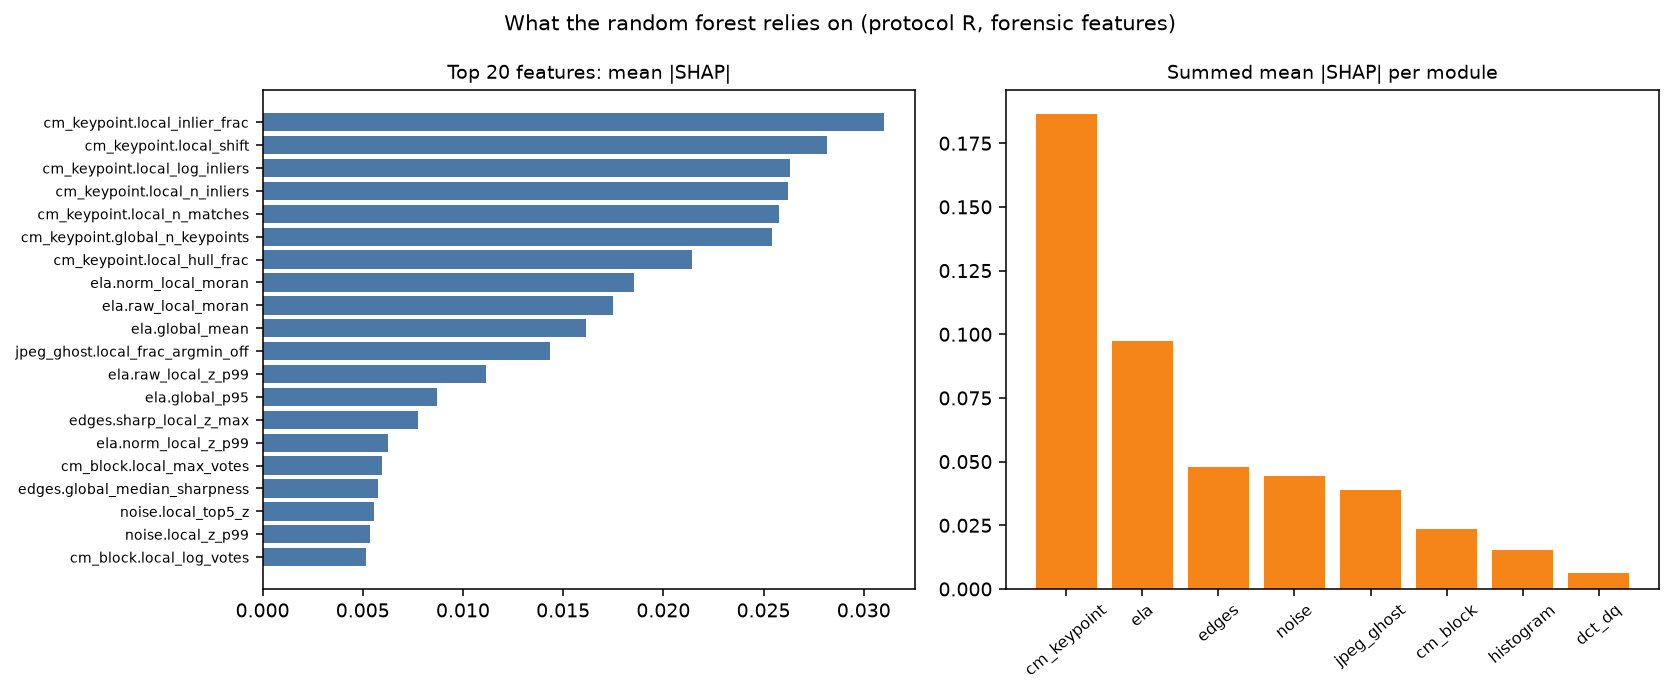
\includegraphics[width=0.9\textwidth]{fig_shap_R.png}
\caption{SHAP explanation of the protocol-R random forest on the forensic features. Left: the 20 features with the largest mean $|$SHAP$|$ (dominated by copy-move keypoint and ELA features). Right: mean $|$SHAP$|$ summed per module.}
\label{fig:shap}
\end{figure*}

\subsection{What the Model Relies On}\label{sec:classification-shap}
Fig.~\ref{fig:shap} shows tree SHAP values \cite{lundberg2017shap,lundberg2020tree} under R. Summed mean $|$SHAP$|$ per module is 0.186 for copy-move keypoints, 0.097 for ELA, 0.048 for edges, 0.044 for noise, 0.039 for JPEG ghosts, 0.024 for copy-move blocks, 0.015 for the histogram and 0.006 for DCT. The single most important feature is the keypoint inlier share, followed by the keypoint shift and the inlier count (log and raw); the most important non-keypoint feature is the spatial clustering (Moran's~I \cite{moran1950}) of texture-normalised ELA. These are within-image evidence, consistent with the ablations.

\subsection{Deployed Models and Sources of Optimism}\label{sec:classification-limits}
Only the nested-CV numbers of Tables~\ref{tab:cls-auc} and~\ref{tab:cls-added} are fully out-of-fold; the ablations, calibration, uncertain band, SHAP and the deployed models (retrained on all dev images) are mildly optimistic (Appendix~\ref{app:classification}), and only the test set (Section~\ref{sec:test}) is free of these effects.

\section{Localisation}\label{sec:localisation}

\subsection{Method}\label{sec:localisation-method}
The eight evidence maps of Section~\ref{sec:method} are reduced to $8 \times 8$-pixel cells. Each cell is described by 16 features: the eight evidence values and their $3 \times 3$-cell neighbourhood means, which add context. Three fusions are compared: the mean of the eight maps (no training), logistic regression, and histogram-based gradient boosting \cite{friedman2001gbm,pedregosa2011sklearn} (300 iterations) on the 16 cell features. The learned fusions are trained on about 2.1--2.3 million cells sampled from training images (Appendix~\ref{app:localisation}); a cell is labelled tampered when at least half of it lies inside the mask.

The cell probability map is upsampled bilinearly, thresholded at $t$, cleaned by morphological opening and then closing with elliptical kernels, and stripped of connected components below a minimum area. These parameters are tuned to maximise mean pixel F1 (grids in Appendix~\ref{app:localisation}). To keep the evaluation honest, the validation images are split into two halves by split group; post-processing is tuned on one half and scored on the other, and the halves swap. The fusion models never see validation images; picking the main method and the best single module by these same numbers slightly flatters both.

For the 769 tampered validation images with a valid mask we compute pixel IoU, F1 and MCC of the final mask and the threshold-free pixel ROC-AUC of the probability map; for the 1,124 authentic validation images, the share with any predicted region and the mean predicted area. Baselines are each single module's map with the same tuning, the \emph{whole image} (F1 $= 2a/(1+a)$ for tampered share $a$) and the \emph{oracle} F1 with the best threshold chosen per image (a reference point, not a strict upper bound).

\begin{table}[!t]
\centering
\caption{Localisation on tampered validation images (mean per image; out-of-sample post-processing). GB = gradient boosting, LR = logistic regression.}
\label{tab:loc-methods}
\scriptsize
\setlength{\tabcolsep}{2.5pt}
\begin{tabular}{lcccccccc}
\toprule
 & \multicolumn{4}{c}{Protocol R} & \multicolumn{4}{c}{Protocol B} \\
Method & F1 & IoU & MCC & AUC & F1 & IoU & MCC & AUC \\
\midrule
GB fusion & \textbf{0.185} & 0.119 & \textbf{0.159} & \textbf{0.695} & \textbf{0.260} & \textbf{0.176} & \textbf{0.254} & \textbf{0.806} \\
LR fusion & 0.184 & 0.121 & 0.155 & 0.686 & 0.237 & 0.158 & 0.224 & 0.786 \\
Mean of 8 maps & 0.159 & 0.099 & 0.100 & 0.671 & 0.175 & 0.113 & 0.150 & 0.734 \\
Copy-move kp.\ only & 0.152 & 0.102 & 0.130 & 0.620 & 0.179 & 0.121 & 0.158 & 0.644 \\
Whole image & 0.136 & 0.086 & -- & -- & 0.136 & 0.086 & -- & -- \\
\emph{Oracle thr.\ (GB)} & \emph{0.308} & -- & -- & -- & \emph{0.436} & -- & -- & -- \\
\bottomrule
\end{tabular}
\end{table}

\subsection{Results}\label{sec:localisation-results}
Table~\ref{tab:loc-methods} summarises the methods; the best single module is copy-move keypoints. Learned fusion is clearly better than any single cue: under R, gradient boosting reaches F1 0.185 against 0.152 for the best single module and 0.159 for the plain average (F1 CI\ci{0.168}{0.200}; all CIs in Appendix~\ref{app:localisation}). Under R no single module beats the trivial whole-image baseline by much, while the combination does; under B the gap is wider (0.260 vs 0.179) and copy-move keypoints alone already beat that baseline clearly. Protocol B localises better than R (F1 0.260 vs 0.185; pixel AUC 0.806 vs 0.695) because the compression modules still see the pasted region's different compression history, which resampling largely removes; for localisation this within-image evidence is genuine (Section~\ref{sec:params}), unlike the global shortcut of Section~\ref{sec:leakage}.

Absolute scores are low; the median tampered region covers 3\% of the image. The oracle F1 (0.31 under R, 0.44 under B) shows that a perfect per-image threshold would raise F1 by about 1.7$\times$, suggesting that much of the gap lies in choosing the threshold for each image rather than in ranking the pixels. By tampered area (R), F1 rises from 0.034 below 1\% to 0.309 above 5\% (Appendix~\ref{app:localisation}); very small regions are essentially not localised. By forgery type (R), copy-move reaches F1 0.204 and splicing 0.152 (B: 0.302 and 0.184), consistent with Section~\ref{sec:classification}. The failure modes (examples in Fig.~\ref{fig:loc-examples}, Appendix~\ref{app:localisation}) are tiny regions, where the probability peak lands elsewhere; large uniform pasted areas (sky, water) with little texture for any module; and textured authentic regions that attract spurious evidence.

\subsection{Gating With the Image Classifier}\label{sec:localisation-gating}
On authentic images the fused mask is rarely empty (a region on 89\% of authentic validation images under R), so the system shows the mask only when the calibrated image-level verdict (Section~\ref{sec:classification}) is not ``authentic''; this cuts the share of authentic images with a false region from 89\% to 42\% under R and from 71\% to 10\% under B, at a small cost in tampered-image F1 (0.186 $\to$ 0.175 under R; Appendix~\ref{app:localisation}).

\emph{Limitations.} Tuning and evaluation use disjoint halves of the same validation set, and the deployed parameters (Appendix~\ref{app:localisation}) are tuned on all of it, so only the test set (Section~\ref{sec:test}) gives a fully independent estimate. The $8 \times 8$ cells limit boundary accuracy (not quantified separately), and tampered images without a valid mask are excluded from scoring.

\section{Test-Set Results and Error Analysis}\label{sec:test}

\subsection{Protocol}\label{sec:test-protocol}
The test split (1,892 images: 1,123 authentic, 769 tampered; 1,092 split groups, none shared with the
development set) was frozen when the splits were made (Section~\ref{sec:leakage}). It was used \emph{once} for the
headline evaluation (run~\#1) and afterwards only for post-hoc evaluations with the same frozen models (the
robustness and synthetic-forgery experiments of Section~\ref{sec:robustness}) and for the pre-registered, one-time
comparison with an ELA-CNN baseline (Section~\ref{sec:cnn}; new models, evaluated once). Nothing from these
experiments was fed back into any model or setting, and each use is recorded in the same run log.

All classifiers, calibrated models and localisers were frozen during development, and the run was guarded by dry
runs, an independent review, a preflight check and a fingerprinted audit record (Appendix~\ref{app:test}).
Confidence intervals are 95\,\% group-bootstrap intervals (1,000 resamples of test split groups).

\subsection{Classification}\label{sec:test-classification}
Table~\ref{tab:test-auc} and Fig.~\ref{fig:roc-test} show that the development estimates hold on unseen data.
Every test AUC is within 0.02 of its cross-validated development estimate (within 0.015 for all random-forest
rows), and every dev estimate falls inside the corresponding test CI (R forensic: dev 0.795, test
0.805\ci{0.779}{0.831}). There is no sign of overfitting to the development set, despite the feature tuning and
model selection done on it.

The central claim is confirmed on test (Table~\ref{tab:test-added}). Under the strict protocol R, the forensic
features beat all global shortcuts combined (0.805 vs 0.712). Added on top of them, they raise AUC by
+0.103\ci{0.076}{0.129}; the purely within-image features alone add +0.083\ci{0.048}{0.116}. Under B the gains
are smaller but still significant (+0.050; local only +0.022\ci{0.003}{0.040}). Protocol A again shows the leak:
on the released files, shortcuts alone reach test AUC 1.000 and forensic features add nothing. RF and SVM cannot
be told apart on the forensic features (McNemar, R: 119 vs 115 discordant, $p=0.84$; B: $p=0.88$).
AUC is the primary metric because the classes are imbalanced (59/41 authentic/tampered) and the operating point
of the deployed detector is set by calibration and abstention (Section~\ref{sec:test-deployed}); for completeness,
Table~\ref{tab:test-threshold} gives the threshold metrics of the forensic random forest at probability 0.5.



\begin{table*}[t]
\centering
\caption{Test ROC-AUC [95\,\% CI], with the development estimate (Section~\ref{sec:classification}) for
comparison.}\label{tab:test-auc}
\footnotesize
\begin{tabular}{lcccccc}
\toprule
Features & R: RF, test & R: RF, dev & R: SVM, test & B: RF, test & B: RF, dev & A: RF, test \\
\midrule
Shortcuts                  & 0.712\ci{0.682}{0.746} & 0.721 & 0.753 & 0.886 & 0.876 & \textbf{1.000} \\
Forensic, local only       & 0.796\ci{0.769}{0.821} & 0.781 & --    & 0.909 & 0.902 & 0.963 \\
\textbf{Forensic, local + global} & \textbf{0.805\ci{0.779}{0.831}} & 0.795 & 0.809 & \textbf{0.920} & 0.910 & 0.981 \\
Forensic + shortcuts       & 0.815\ci{0.789}{0.840} & 0.810 & 0.829 & 0.936 & 0.926 & 1.000 \\
\bottomrule
\end{tabular}

\vspace{3mm}
\caption{Test added value over the shortcuts (paired group bootstrap, $\Delta$AUC [95\,\% CI]).}\label{tab:test-added}
\begin{tabular}{lcccc}
\toprule
Contrast & R: RF & R: SVM & B: RF & A: RF \\
\midrule
(Forensic + shortcuts) $-$ shortcuts        & \textbf{+0.103\ci{0.076}{0.129}} & +0.077\ci{0.054}{0.099} & +0.050\ci{0.036}{0.063} & +0.000 \\
Forensic (local + global) $-$ shortcuts     & +0.093\ci{0.059}{0.125} & +0.056\ci{0.026}{0.085} & +0.033\ci{0.017}{0.049} & $-$0.019 \\
Forensic (local only) $-$ shortcuts         & \textbf{+0.083\ci{0.048}{0.116}} & -- & +0.022\ci{0.003}{0.040} & $-$0.037 \\
\bottomrule
\end{tabular}
\end{table*}

\begin{table}[t]
\centering
\caption{Test metrics at threshold 0.5 (forensic features, local + global, random forest; tampered is the positive
class).}\label{tab:test-threshold}
\footnotesize
\setlength{\tabcolsep}{4pt}
\begin{tabular}{lccccc}
\toprule
 & Accuracy & Precision & Recall & F1 & Balanced acc. \\
\midrule
R & 0.749 & 0.756 & 0.567 & 0.648 & 0.721\ci{0.695}{0.748} \\
B & 0.850 & 0.813 & 0.819 & 0.816 & 0.845\ci{0.826}{0.863} \\
\bottomrule
\end{tabular}
\end{table}

\begin{figure}[t]
\centering
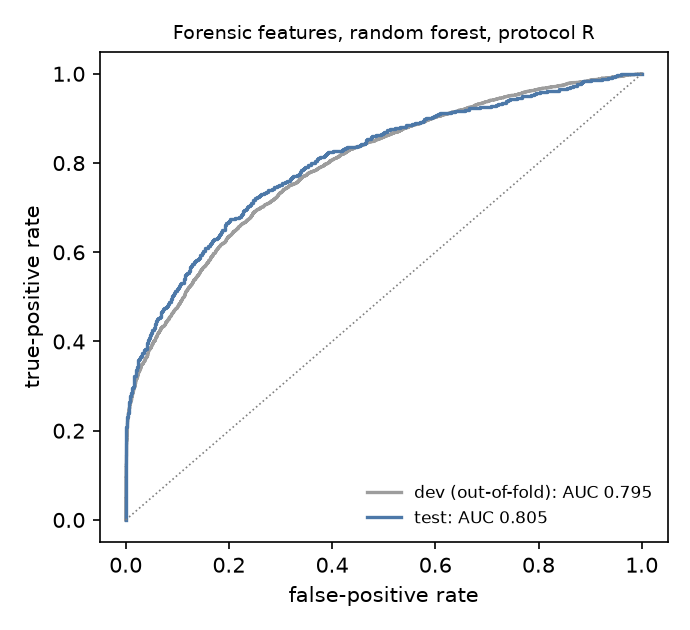
\includegraphics[width=\columnwidth]{fig_roc_test_R.png}
\caption{ROC curves of the forensic random forest under protocol R: development out-of-fold (AUC 0.795) and
the one-time test evaluation (AUC 0.805). The two curves nearly coincide.}
\label{fig:roc-test}
\end{figure}

\subsection{The Deployed Detector}\label{sec:test-deployed}
The deployed detector (protocol R, calibrated, uncertain band $0.5\pm0.24$) behaves on test as it did in
development: it judges 51.8\,\% of the images (dev out-of-fold 51\,\%), with accuracy 0.858 (0.855) and balanced
accuracy 0.809 (0.810) on the judged images, and an expected calibration error of 0.019 (0.009; binned ECE rises
on smaller samples: test 1,892, dev about 10.7k). Table~\ref{tab:test-deployed} gives its verdicts. A ``tampered''
verdict is right 94\,\% of the time (222/235); an ``authentic'' verdict is right 83\,\% of the time (619/745),
because a missed forgery (126) is more common than a false alarm (13). Under B (band $\pm0.04$), 95.7\,\% of
images are judged, with accuracy 0.869 and balanced accuracy 0.853.

\begin{table}[t]
\centering
\caption{Verdicts of the deployed detector on the 1,892 test images (R, band $0.5\pm0.24$).}\label{tab:test-deployed}
\footnotesize
\begin{tabular}{lccc}
\toprule
True class & Authentic & Tampered & Uncertain \\
\midrule
Authentic (1,123) & 619 & 13  & 491 \\
Tampered (769)    & 126 & 222 & 421 \\
\bottomrule
\end{tabular}
\end{table}

\subsection{Localisation}\label{sec:test-localisation}
Table~\ref{tab:test-loc} reports the deployed localiser with frozen post-processing on the 766 test tampered
images with a valid mask. Under R, test localisation matches validation (F1 0.198 vs 0.185); under B it is
\emph{higher} than validation (0.308 vs 0.260, above the test CI); the cause was not investigated. The learned
fusion beats both the best single cue and the plain average; paired test differences in F1 are, under R,
+0.023\ci{0.009}{0.037} over keypoints and +0.029\ci{0.013}{0.045} over the average, and under B
+0.096\ci{0.076}{0.114} and +0.101\ci{0.080}{0.120}. Gating the map by the image verdict reduces the share of
authentic images showing a false region from 89\,\% to 43\,\% (R) and from 73\,\% to 9\,\% (B), at the cost of
tampered F1 falling from 0.198 to 0.189 (R) and from 0.308 to 0.267 (B).

\begin{table}[t]
\centering
\caption{Test localisation (766 tampered images with a valid mask; pixel F1 with 95\,\% CI). Baselines use
post-processing tuned on validation.}\label{tab:test-loc}
\footnotesize
\setlength{\tabcolsep}{4pt}
\begin{tabular}{lcc}
\toprule
 & R & B \\
\midrule
\textbf{Pixel F1} & \textbf{0.198\ci{0.179}{0.216}} & \textbf{0.308\ci{0.284}{0.332}} \\
IoU        & 0.128 & 0.210 \\
MCC        & 0.163 & 0.296 \\
Pixel AUC  & 0.714 & 0.829 \\
F1, mean of maps                  & 0.169 & 0.208 \\
F1, copy-move keypoints only      & 0.174 & 0.212 \\
F1, whole image                   & 0.135 & 0.135 \\
F1, validation (Sec.~\ref{sec:localisation}) & 0.185 & 0.260 \\
\midrule
F1, tampered area $<1$\,\%   & 0.040 & 0.123 \\
F1, tampered area 1--5\,\%   & 0.148 & 0.295 \\
F1, tampered area $>5$\,\%   & 0.333 & 0.413 \\
\midrule
F1, copy-move & 0.236 & 0.354 \\
F1, splicing  & 0.129 & 0.226 \\
\bottomrule
\end{tabular}
\end{table}

\subsection{Error Analysis}\label{sec:test-errors}
Under R, missed forgeries (126) were compared with detected ones (222), and false alarms (13) with correct
authentic verdicts (619); images in the uncertain band are excluded. The comparison uses automatically computed
image properties, with Fisher's exact test and a Holm correction~\cite{holm1979} over the 14 distinct tests
(Table~\ref{tab:test-fisher}; examples in Fig.~\ref{fig:failures}).

\begin{table}[t]
\centering
\caption{Missed vs detected forgeries (R): share of each property, ratio, Fisher $p$ and Holm-adjusted
$p$.}\label{tab:test-fisher}
\footnotesize
\setlength{\tabcolsep}{4pt}
\begin{tabular}{lccccc}
\toprule
Property & Missed & Det. & Ratio & $p$ & Holm $p$ \\
\midrule
Splicing                    & 60\,\% & 3\,\%  & \textbf{22$\times$}  & $<$0.001 & $<$0.001 \\
Keypoints, lowest tercile   & 49\,\% & 21\,\% & \textbf{2.4$\times$} & $<$0.001 & $<$0.001 \\
Tampered area $>5$\,\%      & 33\,\% & 57\,\% & 0.57$\times$ & $<$0.001 & $<$0.001 \\
JPEG source (vs TIFF)       & 44\,\% & 31\,\% & 1.4$\times$  & 0.015 & 0.16 \\
Low texture                 & 42\,\% & 34\,\% & 1.2$\times$  & 0.17  & n.s. \\
Flat, saturated, tiny area  & --     & --     & 1.1--1.4$\times$ & $\geq$0.28 & n.s. \\
\bottomrule
\end{tabular}
\end{table}

The causes of missed forgeries, in order of evidence, are as follows. (i)~\emph{Splicing}: the confident
``tampered'' verdicts are almost all copy-move images. Splicing leaves no internal duplicate, and after
resampling its compression and noise traces are weak (splicing vs authentic AUC 0.68 under R, 0.88 under B).
(ii)~\emph{Few keypoints}: the strongest module, copy-move keypoint matching, has little to work with in smooth,
low-detail images. (iii)~\emph{Area}: regions above 5\,\% are under-represented among misses (0.57$\times$), but
tiny regions ($<1$\,\%) are \emph{not} significantly over-represented. JPEG-sourced forgeries look
over-represented (1.4$\times$, $p=0.015$), but this does not survive the Holm correction; this is the residual
format effect first noted in Section~\ref{sec:classification}, and on test it even reverses under B, where
TIFF-sourced forgeries are detected less often (0.77 vs 0.89).

False alarms are only 13, and none of the image-property tags is significant after correction (low-keypoint
images: 0.33$\times$, $p=0.045$, Holm $p=0.45$). The copy-move features point clearly to the cause: \emph{all 13}
false alarms have copy-move keypoint matches that survive RANSAC~\cite{fischler1981ransac} (median 13 inliers), \emph{none} of the 619
correct authentic verdicts has any, and the false alarms also have many keypoints (median 1,500, the detector's
cap, against 732). Most of the eight false alarms in Fig.~\ref{fig:failures} are \emph{self-similar scenes}
(colonnades and pillars, repeated statues and ornaments, a lattice tower, a zebra-patterned sofa, rows of gaming
machines) in which genuinely repeated structure looks like a copy-move, a known weakness of copy-move
detection~\cite{christlein2012eval,wen2016coverage}. The scene descriptions are qualitative ($n=13$), but the inlier counts are
measured.

\begin{figure*}[t]
\centering
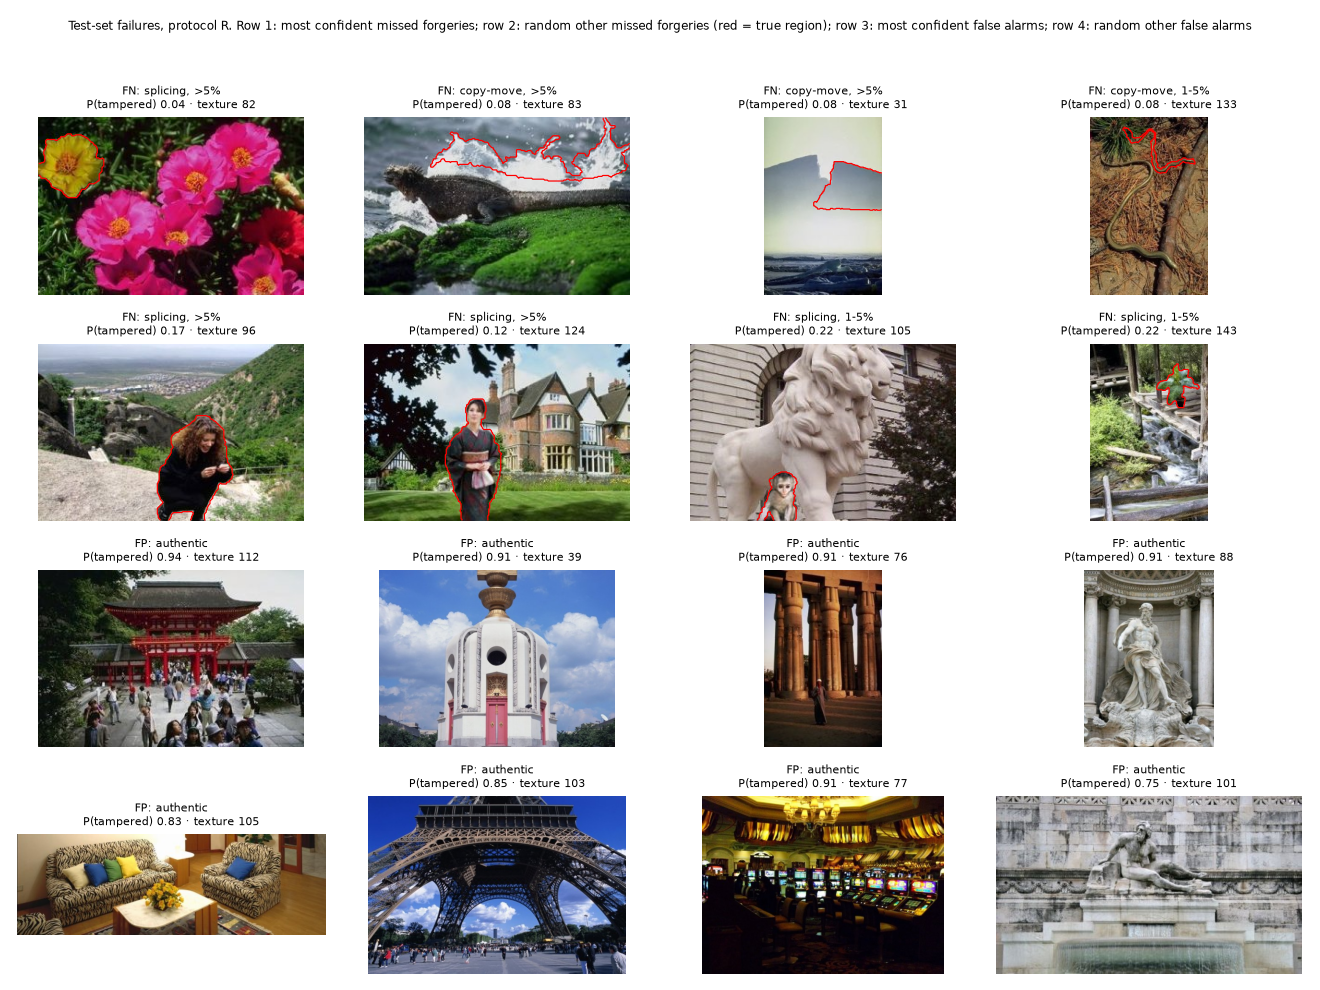
\includegraphics[width=0.9\textwidth]{fig_failures_R.png}
\caption{Test-set failures under protocol R. Row~1: most confident missed forgeries; row~2: random other missed
forgeries (red outline: true region); row~3: most confident false alarms; row~4: random other false alarms. Each
panel gives the forgery type and area class, the calibrated P(tampered) and a texture score. Most false alarms
are self-similar scenes (pillars, statues, a lattice tower, a zebra-patterned sofa, gaming machines).}
\label{fig:failures}
\end{figure*}

\section{Robustness and Generalisation}\label{sec:robustness}
The deployed models are frozen and nothing here is tuned. These experiments re-use the test split \emph{after}
the one-time headline evaluation of Section~\ref{sec:test}, for evaluation only, with nothing fed back; each use
is recorded in the test-run log (two early runs were disclosed in a later note; Appendix~\ref{app:repro}).

\subsection{Robustness to Post-Processing}\label{sec:rob-degrade}
Every test image (1,892) was degraded \emph{before} the protocol was applied: JPEG re-compression at quality
95--50; downscaling by $\times$0.9, $\times$0.75 and $\times$0.5, with the ground-truth mask resized alongside;
Gaussian blur, $\sigma=0.5$--1.5; Gaussian noise, $\sigma=2$--10 grey levels; and a simulated social-media upload
($\times$0.8 downscale, then JPEG quality 70). Table~\ref{tab:rob-degrade} reports
the image-level AUC of the deployed forest and the pixel F1 of the deployed localiser (all conditions are plotted
in Fig.~\ref{fig:robustness}, Appendix~\ref{app:robustness}).

\begin{table}[t]
\centering
\caption{Image AUC (pixel F1) of the frozen detector on the degraded test set.}\label{tab:rob-degrade}
\footnotesize
\begin{tabular}{lcc}
\toprule
Condition & Protocol R & Protocol B \\
\midrule
Clean               & 0.805 (0.197) & 0.920 (0.308) \\
JPEG Q85            & 0.793 (0.193) & 0.903 (0.306) \\
JPEG Q75            & 0.799 (0.193) & \textbf{0.739} (0.223) \\
JPEG Q50            & 0.781 (0.191) & 0.719 (0.214) \\
Resize $\times$0.75 & 0.768 (0.174) & 0.747 (0.170) \\
Resize $\times$0.5  & \textbf{0.693} (0.126) & 0.698 (0.121) \\
Blur $\sigma=1.5$   & 0.764 (0.201) & 0.754 (0.203) \\
Noise $\sigma=10$   & 0.794 (0.197) & 0.803 (0.181) \\
Social upload       & \textbf{0.762} (0.176) & \textbf{0.721} (0.185) \\
\bottomrule
\end{tabular}
\end{table}


Protocol R is robust to re-compression and noise: its AUC stays within 0.03 of the clean value down to JPEG
quality 50 and noise $\sigma=10$, and its localisation F1 hardly changes. R already discards the grid-bound
compression traces, so its evidence (copy-move keypoints, texture-normalised ELA, edges) does not depend on them.
Strong downscaling ($\times$0.5) is its main weakness (AUC 0.69, F1 0.13): smaller images leave fewer keypoints
and blocks.

Protocol B's advantage is fragile. B survives a re-save at quality 95 or 85 (0.900, 0.903; 85 is B's own
re-encode quality), but at a lower quality its clean AUC (0.920) falls below protocol R's: 0.739 at Q75, 0.772 at
Q65 (the decline is not monotonic) and 0.719 at Q50. Under blur, noise or downscaling, B's advantage over R largely
disappears; B stays at most about 0.02 ahead (e.g.\ 0.820 vs 0.802 under noise $\sigma=2$). B's extra signal is
the within-image compression history (Section~\ref{sec:params}), and any further lossy processing overwrites it.
A simulated social-media upload costs about 0.04 AUC under R (0.805 $\to$ 0.762) and 0.20 under B
(0.920 $\to$ 0.721). For images that have been shared online the strict protocol is the realistic setting, which
supports choosing R as the main protocol, a choice Section~\ref{sec:classification} made on other grounds (its
pre-registered rule).

\subsection{Synthetic Forgeries with Known Masks}\label{sec:rob-synthetic}
From the test set's authentic images we generated 480 forgeries with exact masks (tampered regions cover a median
6\,\% of the image, range 0.2--22\,\%), 120 of each kind: hard-edged splices (a random region cut from another
authentic image), seamless splices (the same, blended in with Poisson cloning~\cite{perez2003poisson}), plain
copy-moves (a translated copy of a region) and rotated and scaled copy-moves ($\pm20^\circ$, $\times$0.85--1.15).
A further 240 untouched authentic images, never used as hosts or donors, serve as negatives. All images were
saved losslessly and evaluated as made and after a simulated social-media upload. Mask definitions are given in
Appendix~\ref{app:robustness}.

\begin{table*}[t]
\centering
\caption{Synthetic forgeries: AUC against the 240 untouched authentic images [95\,\% CI], share judged
``tampered'', and pixel F1 (for copy-moves also F1 against source $\cup$ copy, in parentheses). False alarms on the
untouched images: 1.2\,\% (R), 8.8\,\% (B).}\label{tab:rob-synthetic}
\footnotesize
\begin{tabular}{lccccc}
\toprule
Kind & R: AUC & R: detected & R: F1 (source $\cup$ copy) & B: AUC & B: F1 (source $\cup$ copy) \\
\midrule
Splice, hard edge          & 0.569\ci{0.508}{0.629} & 1\,\%  & 0.108 & 0.570 & 0.158 \\
Splice, seamless           & 0.552\ci{0.487}{0.609} & 2\,\%  & 0.079 & 0.551 & 0.225 \\
Copy-move, shift           & \textbf{0.885}\ci{0.830}{0.926} & 73\,\% & 0.376 (\textbf{0.597}) & 0.937 & 0.497 (0.703) \\
Copy-move, rotate + scale  & \textbf{0.896}\ci{0.857}{0.934} & 63\,\% & 0.360 (\textbf{0.571}) & 0.908 & 0.484 (0.653) \\
After a social upload (all kinds) & 0.693 & 27\,\% & 0.182 & 0.687 & 0.222 \\
\bottomrule
\end{tabular}
\end{table*}

Copy-moves are found, including rotated and scaled ones (Table~\ref{tab:rob-synthetic}: AUC 0.89--0.94, F1
0.36--0.50): mirror-aware, scale- and rotation-invariant keypoint matching does what it was designed for.
Fig.~\ref{fig:synthetic} shows that the localiser marks \emph{both} the source and the pasted copy. The ground
truth marks only the copy, so pixel F1 understates copy-move localisation; scored against source $\cup$ copy, F1
rises to 0.60/0.57 under R and 0.70/0.65 under B (shift / rotate + scale).

Splices between two CASIA authentic photos are essentially undetectable (AUC 0.55--0.57; the CI for seamless
splices includes 0.5). This is consistent with the test-set error analysis, where missed forgeries were mostly
splices (Section~\ref{sec:test}), while CASIA's own splices remain more detectable (AUC 0.68 under R). Here the
host and donor share the same kind of camera JPEG history, noise level and processing, so there is no compression,
noise or sharpness inconsistency for the modules to detect; CASIA's own splices are detectable to the extent that
their pasted content differs in such traces, and more so under B. Seamless blending removes the hard edge, yet even
the hard-edged splices are rarely flagged: edge sharpness alone is not enough evidence. Social-media processing
weakens detection (overall AUC 0.725 $\to$ 0.693 under R), with losses spread over the kinds: seamless splices
$-$0.051 (to chance, 0.501), rotated/scaled copy-moves $-$0.048, shifted copy-moves $-$0.024 and hard-edged
splices $-$0.005.

\begin{figure}[t]
\centering
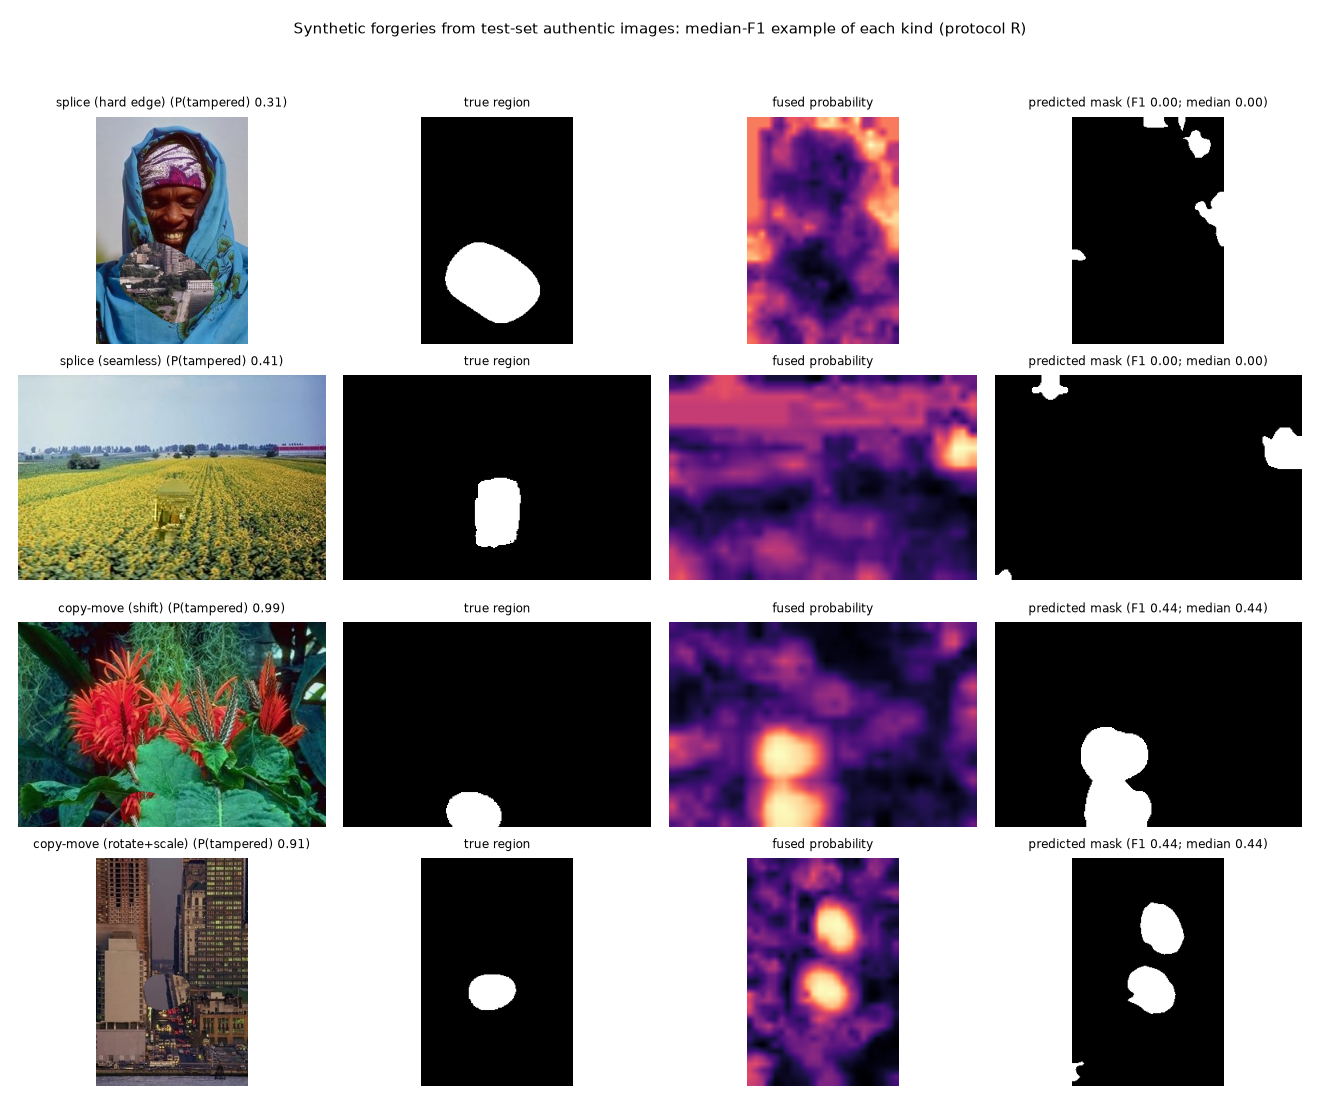
\includegraphics[width=\columnwidth]{fig_synthetic_examples.png}
\caption{Synthetic forgeries from test-set authentic images, median-F1 example of each kind under protocol R
(rows: hard-edged splice, seamless splice, shifted copy-move, rotated and scaled copy-move). Columns: forged image,
true region, fused probability map, predicted mask. For copy-moves the localiser marks both the source and the
copy, whereas the ground truth marks only the copy; the splices are missed.}
\label{fig:synthetic}
\end{figure}

\subsection{Cross-Dataset Test: MICC-F220}\label{sec:rob-micc}
MICC-F220~\cite{amerini2011sift} (used for non-commercial research) contains 110 copy-move forgeries and 110
originals, with larger images than most of CASIA, and is labelled at image level only. The forgeries come from only
11 scenes, each with 10 attack variants (translation, rotation, scaling and combinations), so the AUC rests on 11
forged scenes; the other 99 originals have no forged version. In the bootstrap, each scene's original and its
forgeries form one group.

\begin{table}[t]
\centering
\caption{Cross-dataset evaluation on MICC-F220 without retraining (CM: copy-move keypoint matches).}\label{tab:rob-micc}
\footnotesize
\setlength{\tabcolsep}{4pt}
\begin{tabular}{lcc}
\toprule
 & Protocol R & Protocol B \\
\midrule
AUC [95\,\% CI]                 & \textbf{0.972\ci{0.933}{0.998}} & 0.902\ci{0.767}{0.984} \\
Share of images judged          & 48\,\% & 89\,\% \\
Accuracy on judged          & 0.943 & 0.790 \\
Forgeries judged tampered   & 86\,\% & 88\,\% \\
Originals judged tampered   & 5.5\,\% & 28\,\% \\
Forgeries with CM matches   & 97\,\% & 91\,\% \\
Originals with CM matches   & 23\,\% & 32\,\% \\
\bottomrule
\end{tabular}
\end{table}

The CASIA-trained detector transfers to this unseen copy-move dataset without retraining, with AUC 0.97 under R
(Table~\ref{tab:rob-micc}), driven by the keypoint copy-move module, which finds matches in 97\,\% of the
forgeries. The false-alarm mechanism of Section~\ref{sec:test} appears here too: 23\,\% of the originals contain
copy-move keypoint matches, presumably from repeated structure (not inspected). The calibrated model still keeps
false ``tampered'' verdicts at 5.5\,\% under R, mostly by abstaining: of the 110 originals, 100 fall in the
uncertain band, 4 are judged authentic and 6 tampered, so the judged accuracy of 0.943 comes almost entirely from
the forgeries. B generalises worse: its AUC is 0.90, and the paired group-bootstrap difference is
R $-$ B $=$ +0.069\ci{0.010}{0.172}. Its false-alarm share is 28\,\% against 5.5\,\% for R, although this
comparison uses each protocol's own uncertain band ($\pm0.04$ vs $\pm0.24$). This is consistent with B's reliance
on CASIA-specific compression history.

Other external sets, including COVERAGE~\cite{wen2016coverage}, could not be obtained automatically
(Appendix~\ref{app:robustness}), so a cross-dataset \emph{splicing} test is missing; given
Section~\ref{sec:rob-synthetic}, we expect splicing to be the weaker case.

In summary, under the strict protocol the detector keeps most of its accuracy under re-compression and noise,
generalises to an unseen copy-move dataset and is reliable for copy-move forgeries; its clear limit is splicing
between photographs with the same processing history. Protocol B looks stronger on clean CASIA images, but that
advantage vanishes after a re-save at JPEG quality 75 or below, and on an external dataset.

\section{Comparison With a Deep-Learning Baseline}\label{sec:cnn}

A common approach in the CASIA~v2.0 literature feeds error-level-analysis (ELA) images to a convolutional network and
reports accuracies around 90\%~\cite{sudiatmika2019ela,ali2022recompress}. We built such a baseline, with the same
splits, protocols and frozen test set, to see whether a learned model beats the hand-crafted pipeline once the format
leak is controlled, and whether those high numbers survive that control.

\subsection{Method}\label{sec:cnn-method}

ELA is computed on the image \emph{after} the protocol: the absolute per-channel difference to its JPEG re-save at
quality~90, scaled by 10, clipped to 8~bits and kept at native resolution (examples in Appendix~\ref{app:cnn}). A
ResNet-18~\cite{he2016resnet} with ImageNet weights~\cite{deng2009imagenet} and a single logit is trained on one random
$192\times192$ crop per image per epoch with class-weighted binary cross-entropy and AdamW (details in
Appendix~\ref{app:cnn}); images smaller than a tile are zero-padded, which in ELA space means ``no error''. The image
score pools the logits of overlapping $192\times192$ tiles (stride 96) by their mean or maximum. Only the epoch and the
pooling rule were chosen, by validation AUC; the recipe was then refit on all 10,722 development images, as was the
classical forest. Under R, three seeds differ little on validation (SD 0.008), so one run is representative. Before
the network saw the test split, the comparisons were pre-registered with the SHA-1 of every model; primary were the R
test AUC, the paired difference CNN $-$ classical under R and B, and a fixed rank-average combination of the two
scores. The evaluation ran once. The comparator is the forest on the forensic features (local + global) of
Section~\ref{sec:test}.

\begin{table*}[!t]
\centering
\caption{ELA-CNN vs.\ the classical pipeline: test ROC-AUC [95\% CI] and paired differences (group bootstrap,
1,000 resamples). Classical = random forest on the forensic features.}
\label{tab:cnn-test}
\footnotesize
\begin{tabular}{lccc}
\toprule
 & R & B & A \\
\midrule
ELA-CNN & 0.770\ci{0.744}{0.795} & 0.811\ci{0.788}{0.834} & \textbf{0.994}\ci{0.991}{0.997} \\
Classical & \textbf{0.805}\ci{0.779}{0.831} & \textbf{0.920}\ci{0.905}{0.934} & 0.981\ci{0.975}{0.986} \\
Rank average (CNN, classical) & \textbf{0.824}\ci{0.803}{0.846} & 0.903\ci{0.886}{0.919} & 0.996\ci{0.994}{0.998} \\
\midrule
CNN $-$ classical & $-$0.036\ci{$-$0.067}{$-$0.005} & $-$0.109\ci{$-$0.128}{$-$0.088} & +0.014\ci{0.008}{0.019} \\
CNN $-$ shortcut features (RF) & +0.058\ci{0.030}{0.084} & $-$0.075\ci{$-$0.094}{$-$0.055} & $-$0.005\ci{$-$0.008}{$-$0.003} \\
CNN $-$ shortcut features (SVM) & +0.017\ci{$-$0.011}{0.044} & $-$0.072\ci{$-$0.091}{$-$0.053} & -- \\
Rank average $-$ classical & +0.019\ci{0.003}{0.035} & $-$0.017\ci{$-$0.025}{$-$0.008} & +0.015\ci{0.011}{0.019} \\
\bottomrule
\end{tabular}
\end{table*}

\begin{figure*}[!t]
\centering
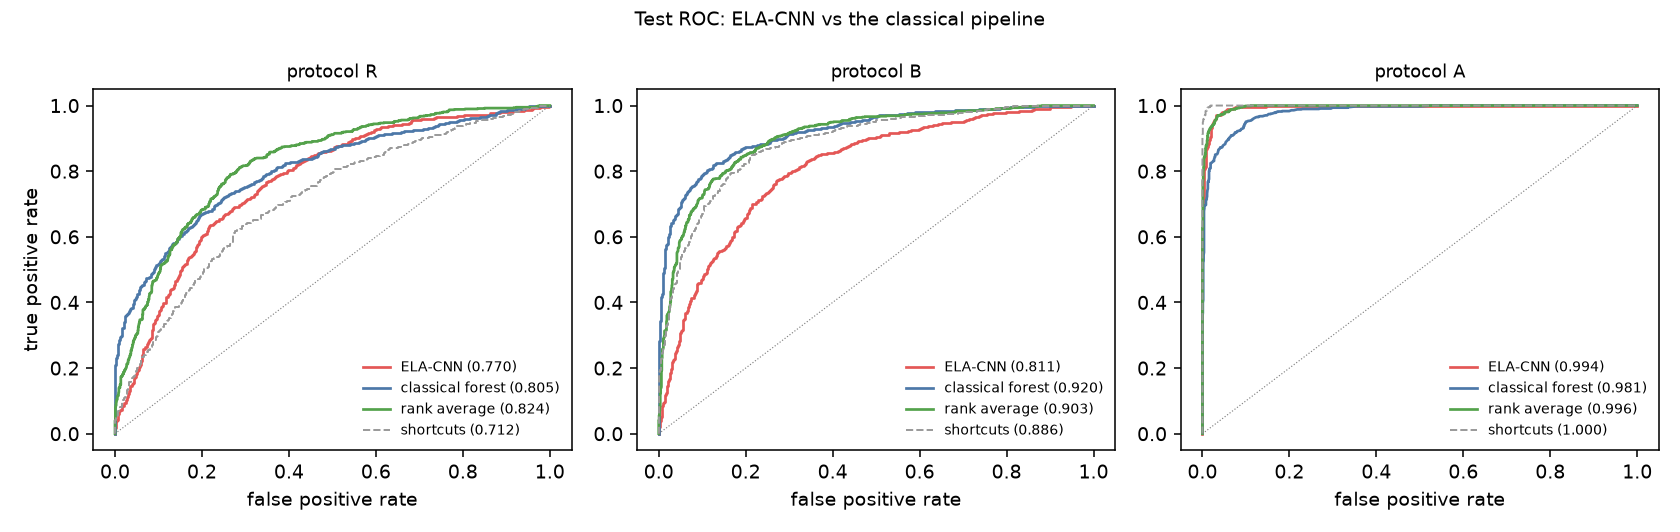
\includegraphics[width=\textwidth]{fig_cnn_roc.png}
\caption{Test ROC curves of the ELA-CNN, the classical forest, their rank average and the shortcut features under
protocols R, B and A (AUC in the legends). Only on the files as released (A) does the CNN reach a very high AUC (0.994),
and there the shortcut features alone reach 1.000.}
\label{fig:cnn-roc}
\end{figure*}

\subsection{Test results}\label{sec:cnn-test}

Table~\ref{tab:cnn-test} and Fig.~\ref{fig:cnn-roc} give the results. With a Holm correction~\cite{holm1979} over the
four primary paired comparisons (CNN $-$ classical and rank average $-$ classical, under R and B), both R results stay
significant (adjusted $p=0.036$ each; unadjusted 0.026 and 0.018, bootstrap $p$-values); the B results have $p<0.002$.
The two R differences are significant on this test set but small, and not adjusted for variation between training
runs, which the test CIs do not include.

\emph{Under the strict protocols the classical pipeline wins.} Under R the CNN is 0.036 below the forensic forest. It
beats the shortcut features' random forest (+0.058) but is not significantly better than their SVM (0.753). Since the
CNN can also see global cues such as the overall ELA level and, through max pooling, image size, we cannot show that
it learns more than the global shortcuts do~\cite{geirhos2020shortcut}. Under B the gap widens to 0.109 and the CNN
falls below B's global shortcuts (0.811 vs.\ 0.886): B keeps within-image compression traces that the DCT, ghost
and ELA modules measure explicitly, and the CNN exploits them less well.

\emph{On the files as released (A)} the CNN reaches AUC 0.994 (the literature reports ${\sim}$90\% accuracy on these
files), while the shortcut features alone reach 1.000 on the same files: the leak alone gives such
a score. It is visible in ELA itself (Fig.~\ref{fig:cnn-ela}, Appendix~\ref{app:cnn}) and persists on JPEG files only
(0.995). A plausible explanation, not tested directly: authentic JPEGs mostly use the standard IJG
tables (89\%), tampered ones never do (Section~\ref{sec:dataset}), and ELA is sensitive to the table. This is
incomplete, since the CNN also separates tampered JPEGs from the 126 authentic JPEGs with non-standard tables (AUC
0.971).

\emph{Under R the two approaches are complementary.} Their scores are moderately correlated (Spearman 0.57), and their
rank average reaches 0.824, the highest R AUC among detectors without shortcut features, level with the best model of
Section~\ref{sec:test}, the SVM on forensic + shortcut features (0.829; difference $-$0.005\ci{$-$0.024}{0.014}). Under
B, averaging in the weaker CNN hurts. The combination ranks scores within the evaluation set and cannot score a single
image, so the deployed detector remains the classical one.

\begin{table}[!t]
\centering
\caption{Test AUC under R by forgery type (authentic vs.\ one type) and by natural image size (post-hoc).}
\label{tab:cnn-groups}
\scriptsize
\setlength{\tabcolsep}{4pt}
\begin{tabular}{lccc}
\toprule
 & CNN & Classical & CNN $-$ classical \\
\midrule
Copy-move & 0.778 & 0.874 & $-$0.096\ci{$-$0.125}{$-$0.069} \\
Splicing & 0.755 & 0.682 & +0.073\ci{0.019}{0.128} \\
\midrule
Smaller than $384\times256$ ($n$=21) & 0.702 & 0.615 & +0.087\ci{$-$0.072}{0.260} \\
$384\times256$ ($n$=1,469) & 0.770 & 0.789 & $-$0.019\ci{$-$0.065}{0.026} \\
Larger than $384\times256$ ($n$=402) & \textbf{0.544} & 0.730 & $-$0.186\ci{$-$0.232}{$-$0.139} \\
\bottomrule
\end{tabular}
\end{table}

\subsection{Where each approach wins}\label{sec:cnn-groups}

Table~\ref{tab:cnn-groups} splits the R results. Keypoint matching is much better at copy-move than the CNN, which is
not built to compare distant regions. On splicing, the classical pipeline's main weakness (Section~\ref{sec:test}), the
CNN wins (+0.073), but the global shortcut features reach almost the same AUC (SVM 0.743; forensic + shortcut SVM
0.752), so this edge may come from global compression or size differences between CASIA's spliced and authentic
images rather than from local splice traces. It is still what makes the rank average help.

The pre-registered size check (AUCs within area terciles) is \emph{invalid}: 78\% of the test images are
$384\times256$ in either orientation, and the code broke this tie by row order, which lists authentic images first, so
the terciles were confounded with the label. A post-hoc grouping by natural size replaces it. On standard-size images
the CNN is not significantly different from the forest, though the wide CI does not show equivalence; most of its
deficit comes from larger images, where it is near chance (0.544); the forest, some of whose features also depend on
size, drops less. Larger authentic images receive much higher CNN scores than standard-size ones (mean logit 1.35
vs.\ $-$0.40): the network appears to have learned the ELA statistics of the dominant $384\times256$ images and to
treat others as suspicious (an interpretation; the image sources were not analysed).

\emph{Transfer.} The CNN does not transfer to MICC-F220: AUC 0.529\ci{0.360}{0.700} under R, consistent with chance,
against 0.972 for the classical detector (11 forged scenes, hence the wide CI). Degradation results are in
Appendix~\ref{app:cnn}.

\subsection{Summary and limitations}\label{sec:cnn-summary}

A standard ELA-CNN reaches high scores only on the leaking files. Under R and B it is below the
classical pipeline and not significantly better than a shortcut-feature SVM, but under R its rank average with the
forest matches the best model. Its failure on MICC-F220 is the strongest argument in this study for explicitly modelled
classical cues. Limitations: one architecture and input representation, no search beyond epoch and pooling, a single
validation split, and non-bit-reproducible GPU training. A stronger network, e.g.\ trained end-to-end on RGB with
constrained convolutions~\cite{bayar2016constrained}, might close the gap under R, but would need the same leak
controls.

\section{System and Demonstration}\label{sec:system}

\textbf{Single entry point.} The command line, the batch mode and the interface all call one function,
\texttt{detect()}. It loads the image, applies the protocol, runs the eight modules with the tuned parameters
(Section~\ref{sec:params}), classifies with the calibrated forest, estimates the forgery type, localises with the
learned fusion and gates the mask by the verdict. It refuses a model whose recorded feature parameters or protocol
differ from the current configuration, so no entry point can drift from the evaluated system.

\textbf{Explanations.} Each result carries the exact SHAP contributions (TreeExplainer)~\cite{lundberg2017shap,
lundberg2020tree} of the 82 features to the forest's score, translated into plain language; a unit test checks that
they plus the base value reproduce the forest's probability exactly. The calibrated probability is a monotone
transformation of that score, so the directions carry over but the sizes are not on the probability scale. The verdict
text states the uncertain band (P(tampered) within $0.50\pm0.24$ under R gives no verdict) and the share of test
images in it (48\% under R, 4\% under B); evidence sentences name the strongest evidence and the known false-alarm
cause, repeated real structure mimicking a copy-move (Section~\ref{sec:test}). A PDF report and a JSON record can be
exported.

\textbf{Input preparation.} Every image is validated and normalised before analysis (Appendix~\ref{app:system}).

\begin{figure}[!t]
\centering
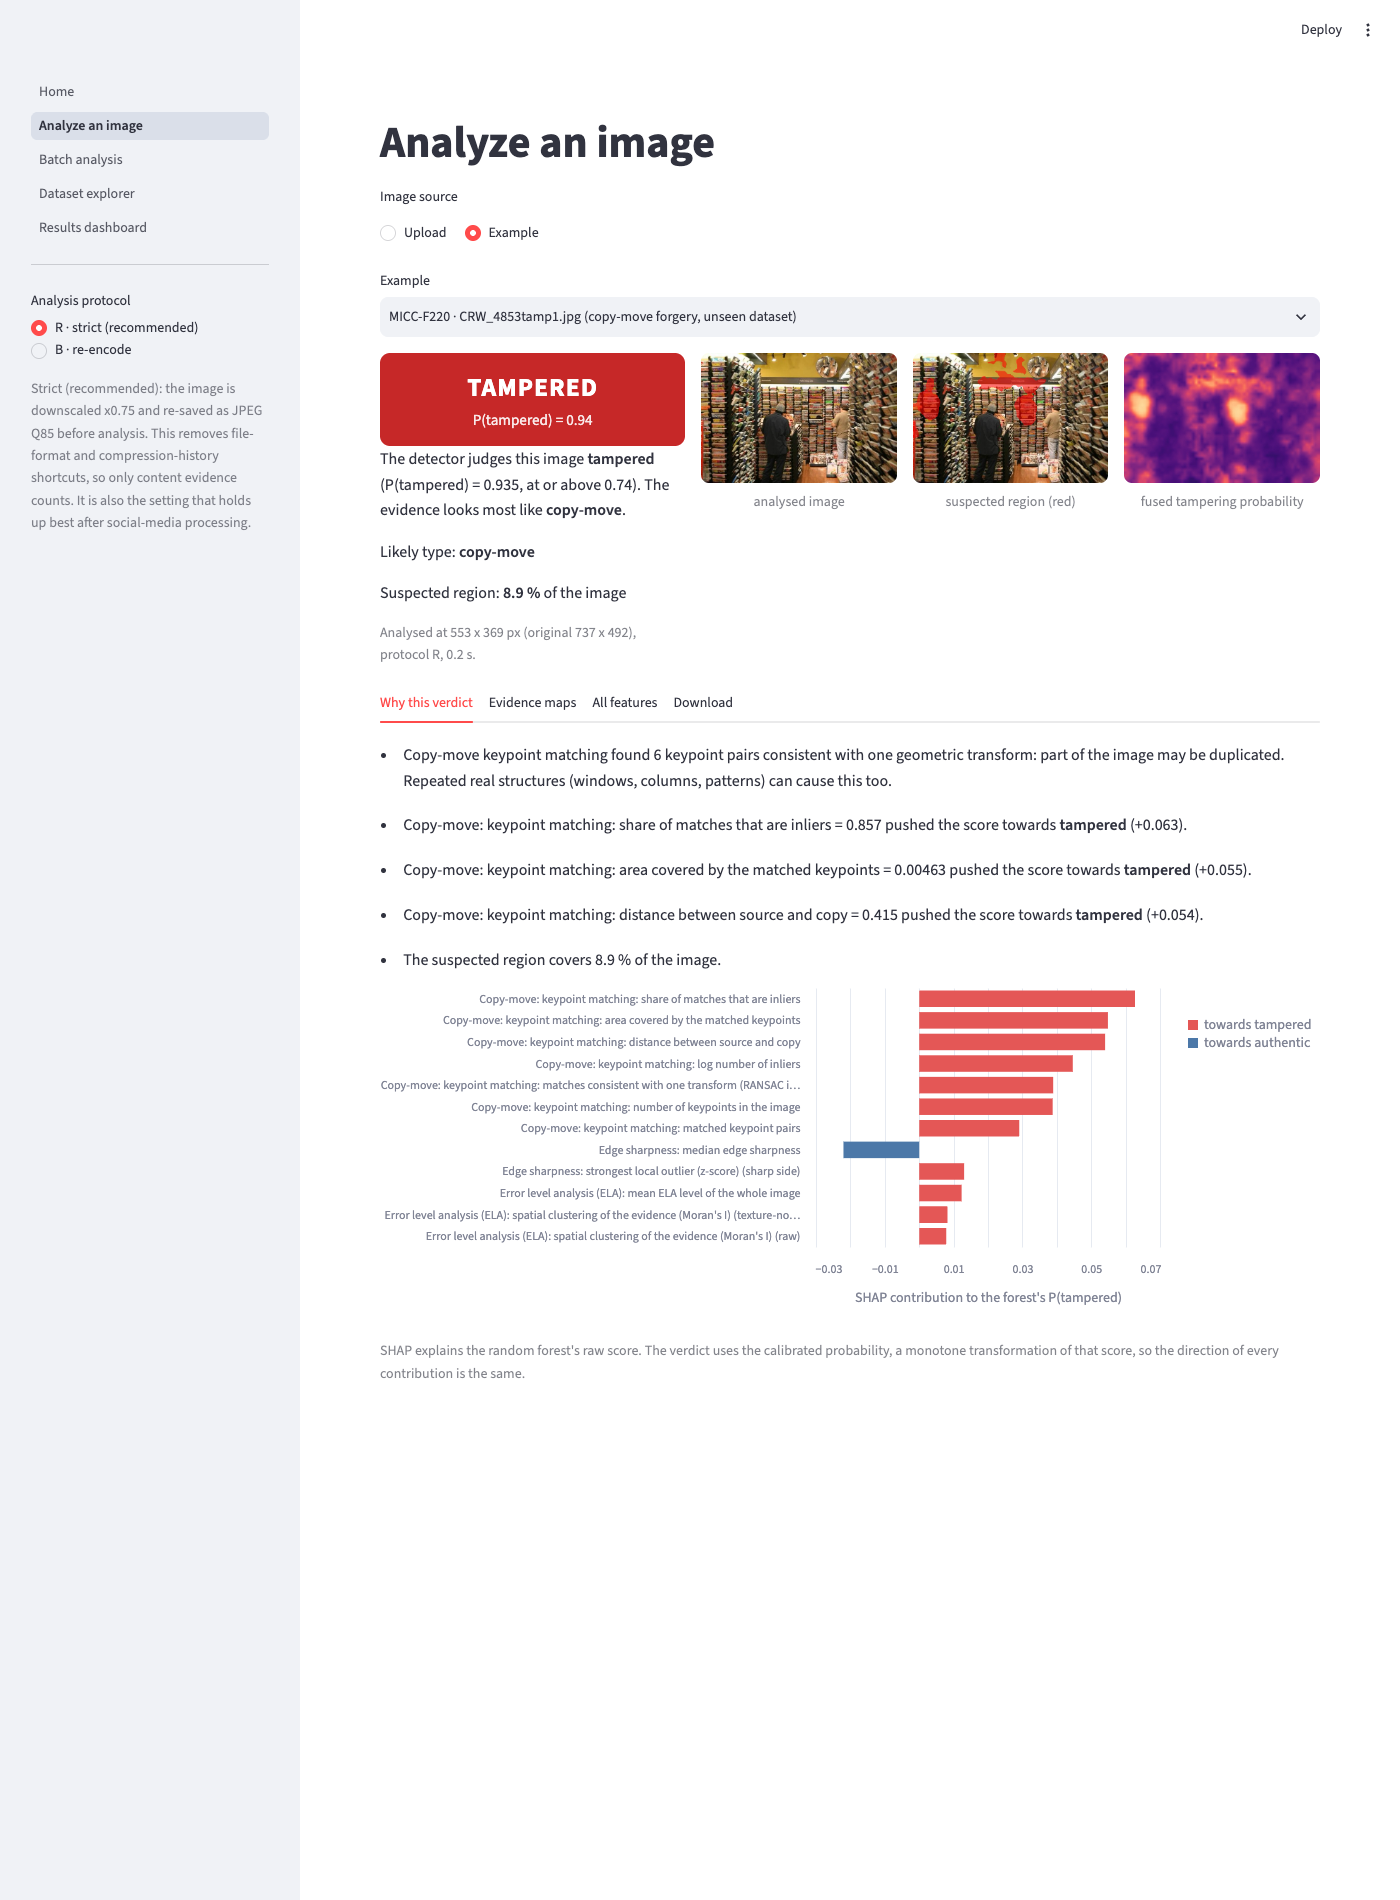
\includegraphics[width=\columnwidth, trim=375 1235 75 340, clip]{fig_ui_analyze.png}
\caption{Result panel of the ``Analyze an image'' page for a MICC-F220 copy-move example under protocol R: verdict
with P(tampered), likely type and size of the suspected region, next to the analysed image, the suspected region (red)
and the fused tampering probability map. Evidence sentences and the per-image SHAP chart follow below it on the page (not shown).}
\label{fig:ui-analyze}
\end{figure}

\textbf{Interface.} A four-page Streamlit application offers (1)~\emph{Analyze an image} (Fig.~\ref{fig:ui-analyze}):
verdict, likely type, suspected region, fused map, explanation, per-technique evidence maps and downloads, with the
protocol chosen in the sidebar (R by default); (2)~\emph{batch analysis} of up to 200 files or a folder, where an
unreadable file does not stop the batch; (3)~a \emph{dataset explorer} whose leak tab shows format and quantisation
tables by class and the shortcut classifiers' balanced accuracy per protocol; (4)~a \emph{results dashboard} that
reads the saved evaluation without recomputing it.

\textbf{Keeping the evaluation honest.} The explorer never lists the test split. CASIA examples are labelled as
training data, since the deployed models were refit on them; MICC-F220 images serve as unseen examples. The home page
states the limits: trained on CASIA, a verdict is evidence, not proof, about half of all images fall in the uncertain
band, and the known weaknesses.

\textbf{Performance and verification.} A CASIA-sized image is analysed in about 0.2~s, and every page is covered by
automated headless tests (Appendix~\ref{app:system}).

\section{Limitations and Conclusion}\label{sec:conclusion}

\textbf{Limitations.}
\begin{itemize}\setlength\itemsep{0pt}
\item \emph{Splicing is the main weakness.} Splices whose host and donor share the same processing history leave
no compression, noise or edge inconsistency; synthetic splices between two CASIA photographs were detected at
close to chance level (Section~\ref{sec:robustness}). Missed test-set forgeries were mostly splices
(Section~\ref{sec:test}).
\item \emph{Self-similar scenes cause false alarms.} Colonnades, lattices and repeated patterns mimic copy-moves.
All 13 confident false alarms on the test set had copy-move keypoint matches that survived RANSAC.
\item \emph{Localisation is coarse.} The fusion works on 8$\times$8 cells, and pixel F1 remains modest (0.198
under R; 0.333 for regions above 5\% of the image). Small regions ($<$1\%) are rarely found.
\item \emph{Limited external validation.} Only one external dataset, MICC-F220, could be obtained, and it contains
copy-moves from 11 scenes only. A cross-dataset splicing test is missing.
\item \emph{Remaining shortcuts.} The protocols remove most, not all, of the leak: under R the shortcut features
still reach AUC 0.712 on test, mainly through image size. We therefore report added value over the shortcuts, not
absolute accuracy alone.
\item \emph{Module limits.}
  \begin{itemize}\setlength\itemsep{0pt}
  \item The DCT periodicity test misses some double-quantisation patterns; it detected about 56\% of simulated
  double compressions.
  \item The keypoint matcher recovers at most one copied region per matching mode.
  \end{itemize}
\item \emph{Baseline scope.} The CNN comparison uses one architecture and one input representation, with less
tuning than the classical system.
\end{itemize}

\textbf{Conclusion.} CASIA~v2.0 as released does not measure what it is meant to measure: its labels can be
predicted from file metadata alone. Once that shortcut is removed and forensic features are required to beat the
cues that remain, an interpretable pipeline of classical DIP techniques still carries genuine tampering evidence:
\begin{itemize}\setlength\itemsep{0pt}
\item \emph{Classification.} Test AUC 0.805 under the strict protocol, +0.103 over the shortcut features.
\item \emph{Abstention.} The calibrated detector judges about half of the images, with 86\% accuracy.
\item \emph{Localisation.} It marks tampered regions and explains every decision with evidence maps and feature
attributions.
\item \emph{Transfer.} It reaches AUC 0.972 on an unseen copy-move dataset (MICC-F220, 11 forged scenes).
\end{itemize}
A standard ELA-CNN, by contrast, reaches its highest score (AUC 0.994) only on the leaking files, where shortcut
features alone reach 1.000. It trails the classical pipeline under both controlled protocols, and on that dataset
its AUC is consistent with chance.

The broader lesson concerns evaluation. Before a high score on a forensic benchmark is taken as evidence of
detection, the benchmark should be checked for shortcuts, and methods should be compared with what those shortcuts
alone achieve. Promising next steps are:
\begin{itemize}\setlength\itemsep{0pt}
\item cues aimed at same-history splices, such as sensor-noise consistency;
\item suppression of copy-move false alarms on repeated structure;
\item a cross-dataset splicing benchmark;
\item learned detectors trained and evaluated under the same leak controls.
\end{itemize}


\balance
\bibliographystyle{IEEEtran}
\bibliography{refs}

\clearpage
\onecolumn
\appendices
% Each section writer may add sections/appendix_<key>.tex; they are included here if present.
\IfFileExists{sections/appendix_repro.tex}{\section{Reproducibility and Audit Trail}\label{app:repro}

\textbf{Code and environment.}
\begin{itemize}\setlength\itemsep{0pt}
\item \emph{Code:} all code is in one Python package (\texttt{src/forgery}), with one script per pipeline step
(\texttt{scripts/}).
\item \emph{Parameters:} every parameter is in \texttt{config.yaml}, and the random seed is fixed at 42.
\item \emph{Software:} Python 3.12 with NumPy, OpenCV, scikit-image, scikit-learn, SHAP, PyTorch/torchvision (for
the CNN baseline only) and Streamlit (for the interface); exact versions are pinned in \texttt{requirements.txt}.
\item \emph{Hardware:} all experiments ran on an Apple M4 laptop with 16\,GB of memory; the CNN was trained on
its GPU through the MPS backend.
\item \emph{Tests:} a test suite of 209 unit, data-invariant and interface tests (\texttt{pytest}) covers the
modules on synthetic forgeries with known regions, the I/O and protocol code, the split invariants, the statistics
and the interface.
\end{itemize}

\textbf{Pipeline.} Table~\ref{tab:repro} lists the steps in order. Each step reads the outputs of earlier steps and
writes its tables and figures to \texttt{results/phase$N$/}; figures are never edited by hand.

\begin{table}[h]
\centering
\caption{Pipeline steps and their outputs}\label{tab:repro}
\scriptsize
\begin{tabular}{lll}
\toprule
Step & Script & Main output \\
\midrule
Dataset audit & \texttt{build\_manifest.py} & \texttt{data/manifest.csv}, \texttt{results/phase1/} \\
Split and leakage study & \texttt{make\_splits.py}, \texttt{run\_leakage\_study.py} & \texttt{data/splits.csv}, \texttt{results/phase2/} \\
Module sanity check & \texttt{phase3\_sanity.py} & \texttt{results/phase3/} \\
Parameter sweeps & \texttt{sweep\_params.py -{}-write-config} & \texttt{config.yaml}, \texttt{results/phase4/} \\
Features and classification & \texttt{extract\_features.py}, \texttt{run\_phase5.py} & \texttt{models/}, \texttt{results/phase5/} \\
Localisation & \texttt{extract\_maps.py}, \texttt{run\_phase6.py}, \texttt{phase6\_gating.py} & \texttt{models/}, \texttt{results/phase6/} \\
One-time test evaluation & \texttt{run\_phase7.py}, \texttt{phase7\_posthoc.py} & \texttt{results/phase7/run\_1/} \\
Robustness, synthetic, MICC-F220 & \texttt{run\_phase7b.py} & \texttt{results/phase7b/} \\
CNN baseline & \texttt{make\_ela.py}, \texttt{run\_phase8.py}, \texttt{phase8\_posthoc.py} & \texttt{models/cnn\_*.pt}, \texttt{results/phase8/} \\
Interface & \texttt{streamlit run app/Home.py} & -- \\
This report & \texttt{build\_report.py} & \texttt{report/*.pdf} \\
\bottomrule
\end{tabular}
\end{table}

\textbf{Frozen split.} The split was frozen before any model was trained. Its SHA-256 hashes are stored in
\texttt{data/test\_split.sha256}:
\begin{itemize}\setlength\itemsep{0pt}
\item test split: \texttt{a437cb81\ldots b0b4}
\item full split: \texttt{6991cc0c\ldots 4468}
\end{itemize}
\texttt{make\_splits.py} refuses to change them unless it is explicitly asked to re-freeze.

\textbf{Test-set use.} Every use of the test split is recorded in \texttt{results/phase7/test\_runs.log}:
\begin{enumerate}\setlength\itemsep{0pt}
\item \emph{Headline evaluation (run~1), 2026-09-24.} The log holds a start record with fingerprints of all source
files and inputs, and a completion record with the hashes of the outputs.
\item \emph{Post-hoc robustness, synthetic and external evaluation (Section~\ref{sec:robustness}), 2026-09-25.} Frozen models,
evaluation only, nothing fed back. Two earlier runs of these experiments, made before the log entry existed, are disclosed in a
note record.
\item \emph{CNN evaluation, 2026-09-27.} New models, evaluated once after a pre-registration that fixed the
comparisons and the model hashes. The log holds start and completion records.
\end{enumerate}
All other analyses of test results read the saved outputs only. Known deviations and their resolutions are listed in
\texttt{report/KNOWN\_ISSUES.md}.

\textbf{Compute.} The complete pipeline, excluding the CNN, runs in a few hours on the laptop above, most of it
spent on feature extraction and the parameter sweeps of Section~\ref{sec:params}; the CNN selection and refit took about 3.5\,h of GPU
time. Analysing a single typical image takes about 0.2\,s.
}{}
\IfFileExists{sections/appendix_dataset.tex}{\section{Dataset Audit Details}\label{app:dataset}

\textbf{Mask names.} 142 mask names differ from their image name: 97 differ only in the S/D letter, 44 differ in the
host or donor id (10 of them use the placeholder id \texttt{xxx00000}), and 1 is named \texttt{\ldots\_gt3.png}.
Matching on the trailing tamper id, which is unique across the dataset, gives every tampered image exactly one mask.

\textbf{Unusable masks (19).} 5 are transposed (width and height swapped: four $256\times384$ masks for
$384\times256$ images, and one $638\times336$ mask for a $336\times638$ image); 12 have other sizes (9 differ from the
image by 1 to 11 pixels, and 3 by 125 to 200 pixels); 2 cover more than 95\% of the image. These 19 images remain in
the classification experiments but are excluded from localisation scoring.

\textbf{Mask verification.} The reference signal is where the tampered image differs from its background image
(blurred absolute grey-level difference $>20$). The background image is the named authentic image that best matches
the area \emph{outside} the mask. It is the host for 5,029 masks and the second-named image for 5, where the ids are
swapped, so the check was possible for 5,034 masks. The median share of mask pixels that differ from the background
(recall) is 0.885, and the median share of changed pixels inside the mask (precision) is 0.991. The 52 masks with
recall $<0.2$ are flagged for inspection but not removed.

\textbf{Which named image is the background?} A tampered file name
\texttt{Tp\_<S|D>\_\ldots\_<id1>\_<id2>\_<n>} names two authentic images. For every tampered image we measured the
share of pixels within 10 grey levels of each named image (sizes must match). For the 1,778 splicing-named images
whose ids differ, \texttt{id1} supplies most pixels in 1,689, \texttt{id2} in 20, and neither in 69 (27 because the
host has a different size, 42 because neither image matches more than half of the pixels). For the 44
copy-move-named images with differing ids, the counts are 37, 3 and 4. We therefore treat \texttt{id1} as the host.
In the 23 images where the second-named image supplies most pixels, 18 are large pastes (the mask, which marks the
pasted region, covers 52--96\% of the frame) and 5 have swapped ids (the pasted region is small, 0.8--6.8\% of the
image, and the unmasked background matches \texttt{id2}, so the two ids appear to be swapped in the file name). All
23 are additionally grouped with the second-named image (Section~\ref{sec:leakage}).
}{}
\IfFileExists{sections/appendix_leakage.tex}{\section{Splits and Shortcut Study: Details}\label{app:leakage}

Table~\ref{tab:leakage-full} extends Table~\ref{tab:leakage} with the ROC-AUC of each shortcut classifier (random
forest, 300 trees, balanced class weights; balanced accuracy is the mean over the five grouped dev folds, with the
standard deviation given for the combined feature set under B and R).

\begin{table}[h]
\centering
\caption{Global shortcut features alone: balanced accuracy (ROC-AUC) per protocol}\label{tab:leakage-full}
\footnotesize
\begin{tabular}{lcccc}
\toprule
Features & A: as released & C: JPEG only & B: re-encoded & R: resampled \\
\midrule
File metadata & \textbf{0.990} (0.999) & \textbf{0.991} (0.996) & 0.508 (0.510) & 0.503 (0.509) \\
Image dimensions & 0.603 (0.642) & 0.597 (0.645) & 0.603 (0.642) & 0.604 (0.643) \\
Naive global ELA & 0.696 (0.778) & 0.678 (0.782) & 0.564 (0.597) & 0.539 (0.556) \\
Compression history & 0.928 (0.981) & 0.955 (0.990) & \textbf{0.789} (0.870) & 0.608 (0.683) \\
All shortcuts & 0.989 (0.999) & 0.986 (0.998) & \textbf{0.797} $\pm$ 0.007 (0.876) & \textbf{0.649} $\pm$ 0.011 (0.720) \\
\bottomrule
\end{tabular}
\end{table}

\textbf{Split construction.} A near-duplicate candidate needs a 64-bit dHash Hamming distance $\leq 8$, and is
confirmed only if the $32\times32$ grey thumbnails have a mean absolute difference $<5$ and a correlation $>0.95$.
dHash alone matched many unrelated photos with smooth gradients; the thumbnail check removes those. With stratified
group $k$-fold assignment (20 bins, seed 42, strata of forgery type $\times$ file format), every stratum is within
0.23 percentage points of its target share, except the 54-image BMP stratum, which is within 1.67. The split is
frozen by SHA-256 hashes of the test file list and of the whole split table.

\textbf{Feature families.} File metadata: format flags, quantisation-table statistics, standard-table flag, bytes
per pixel. Image dimensions: width, height, aspect ratio, megapixels. Naive global ELA: mean, standard deviation
and 95th/99th percentiles of one ELA residual at Q=90. Compression history: global double-quantisation statistics
(histograms of $8\times8$-DCT coefficients at five low frequencies, divided by the last quantisation step) and a
global JPEG-ghost curve (mean re-compression error at Q = 60, 65, \ldots, 95).

\textbf{Re-encode quality for B} (all shortcuts, balanced accuracy): Q=75 gives 0.791, Q=85 gives 0.797, Q=95 gives
0.855.
}{}
\IfFileExists{sections/appendix_method.tex}{\section{Feature Module Details}\label{app:method}

\textbf{DCT double quantisation.} Under protocols B and R the last compression is known (Q85), so the module uses
the exact IJG Q85 quantisation table; a blind estimate of the last quantisation step is used only when it is
unknown (protocol A, or arbitrary input files). Periodicity is tested on the log-histogram of each frequency's
coefficients after removing a quadratic trend. The residual is projected on every candidate period from 2 to half
the histogram range, including fractional periods. The largest normalised power is compared with its
\emph{permutation null}: the same maximum computed after shuffling the residual across bins, 200 times per
histogram. This gives a calibrated p-value whatever the histogram's width or tails, and however many periods are
tried. Periodicity is declared at $p\leq\alpha$, with $\alpha$ tuned in Section~\ref{sec:params}. On dedicated test
cases the false-positive rate at $\alpha = 0.01$ is 0--3\% (0.4\% on real history-free images), against 16--48\%
for an earlier fixed threshold. Genuinely double-compressed test images are flagged at 75\% of frequencies, but
overall detection on simulated double compression is only about 56\%: some regular patterns are missed, e.g.\
$q_1/q_2 = 10/4$ (a period of 2.5 bins) was detected in 0/30 simulations, while 9/4, 7/3 and 8/3 were detected in
30/30. The per-coefficient posterior compares the observed histogram with a uniform one inside a window spanning a
whole number of periods.

\textbf{Blind quantisation-step estimator.} The estimator picks the largest step that is a local maximum of the
integer-fit score and reaches 80\% of what pixel-rounding noise allows ($\sigma = 0.5$, relaxed to 1.0 for
saturated images). When the first step is an exact multiple of the last (e.g.\ 9 and 3), double compression cannot
be detected blindly at that frequency.

\textbf{Mirrored copies.} Several CASIA copy-moves are horizontally flipped duplicates, which neither SIFT
descriptors nor block DCT features match directly. Both detectors therefore also match against the mirrored image.
For keypoints, descriptors are recomputed at the mirrored keypoint positions. For blocks, the shift measured in
(image, mirror) coordinates is constant for a mirrored copy, so ordinary shift voting still applies; the mirrored
image's block grid is offset so that it aligns with the image's block grid.

\textbf{Pair orientation.} A translation has a direction, so direct keypoint pairs are oriented left-to-right
before RANSAC. Unoriented pairs split one true copy into two opposite transforms, and RANSAC then rejected genuine
copies. Mirrored pairs are oriented left-to-right as well: a mirrored copy with a vertical offset is a glide
reflection, whose inverse is a different transform, so the same split would occur. One RANSAC fit is run per
matching mode (direct and mirrored), so the keypoint detector recovers at most one copied region per mode.

\textbf{Verification.} The synthetic forgeries with a known region are: for ELA and the histogram module, an
uncompressed region inside a Q60 image; for noise, a noisier region; for JPEG ghosts, a region previously saved at
Q60 inside a Q90 image, re-saved at Q95; for DCT, a single-compressed region inside a double-compressed image; for
edges, an unblurred region in a blurred image of the same content; and for copy-move, plain and mirrored copies.
Contract tests cover tiny ($8\times8$), narrow ($200\times13$), flat and black images, and check determinism. The
modules are implemented in \texttt{src/forgery/features/} and tested in \texttt{tests/test\_features.py}; the
synthetic tests run both with the default parameters and with the tuned parameters from \texttt{config.yaml}.
}{}
\IfFileExists{sections/appendix_params.tex}{\section{Chosen Parameters and Sweeps}\label{app:params}

Table~\ref{tab:params-chosen} lists the parameters chosen by the coordinate-ascent sweeps of
Section~\ref{sec:params} (protocol B, validation sample); changes from the default are in bold. Fig.~\ref{fig:sweeps}
shows the sweep curves. The sweeps were run with \texttt{scripts/sweep\_params.py}; the chosen values are stored in
\texttt{config.yaml}.



\begin{table}[!ht]
\centering
\caption{Chosen parameters per module (changes from the default in bold)}\label{tab:params-chosen}
\footnotesize
\begin{tabular}{ll}
\toprule
Module & Chosen parameters \\
\midrule
ELA & $\mathbf{q = 85}$, block 8, \textbf{texture} $\mathbf{c = 16}$ \\
Patch-histogram $\chi^2$ & $\mathbf{q = 75}$, \textbf{patch 16}, 16 bins \\
Noise level & Immerk{\ae}r, block 8, \textbf{edge quantile 0.8, min.\ block std 2} \\
JPEG ghosts & block 16, \textbf{min.\ std 4} \\
DCT double quantisation & \textbf{15 frequencies}, $\boldsymbol{\alpha = 0.05}$ (permutation-test level) \\
Edge sharpness & \textbf{Canny 30 / 90}, block 16 \\
Copy-move keypoints & SIFT, ratio 0.6, contrast 0.01, mirror matching (defaults kept) \\
Copy-move blocks & tol 1.5, min.\ std 4, 8 votes, mirror matching (defaults kept) \\
\bottomrule
\end{tabular}
\end{table}

\begin{figure}[p]
\centering
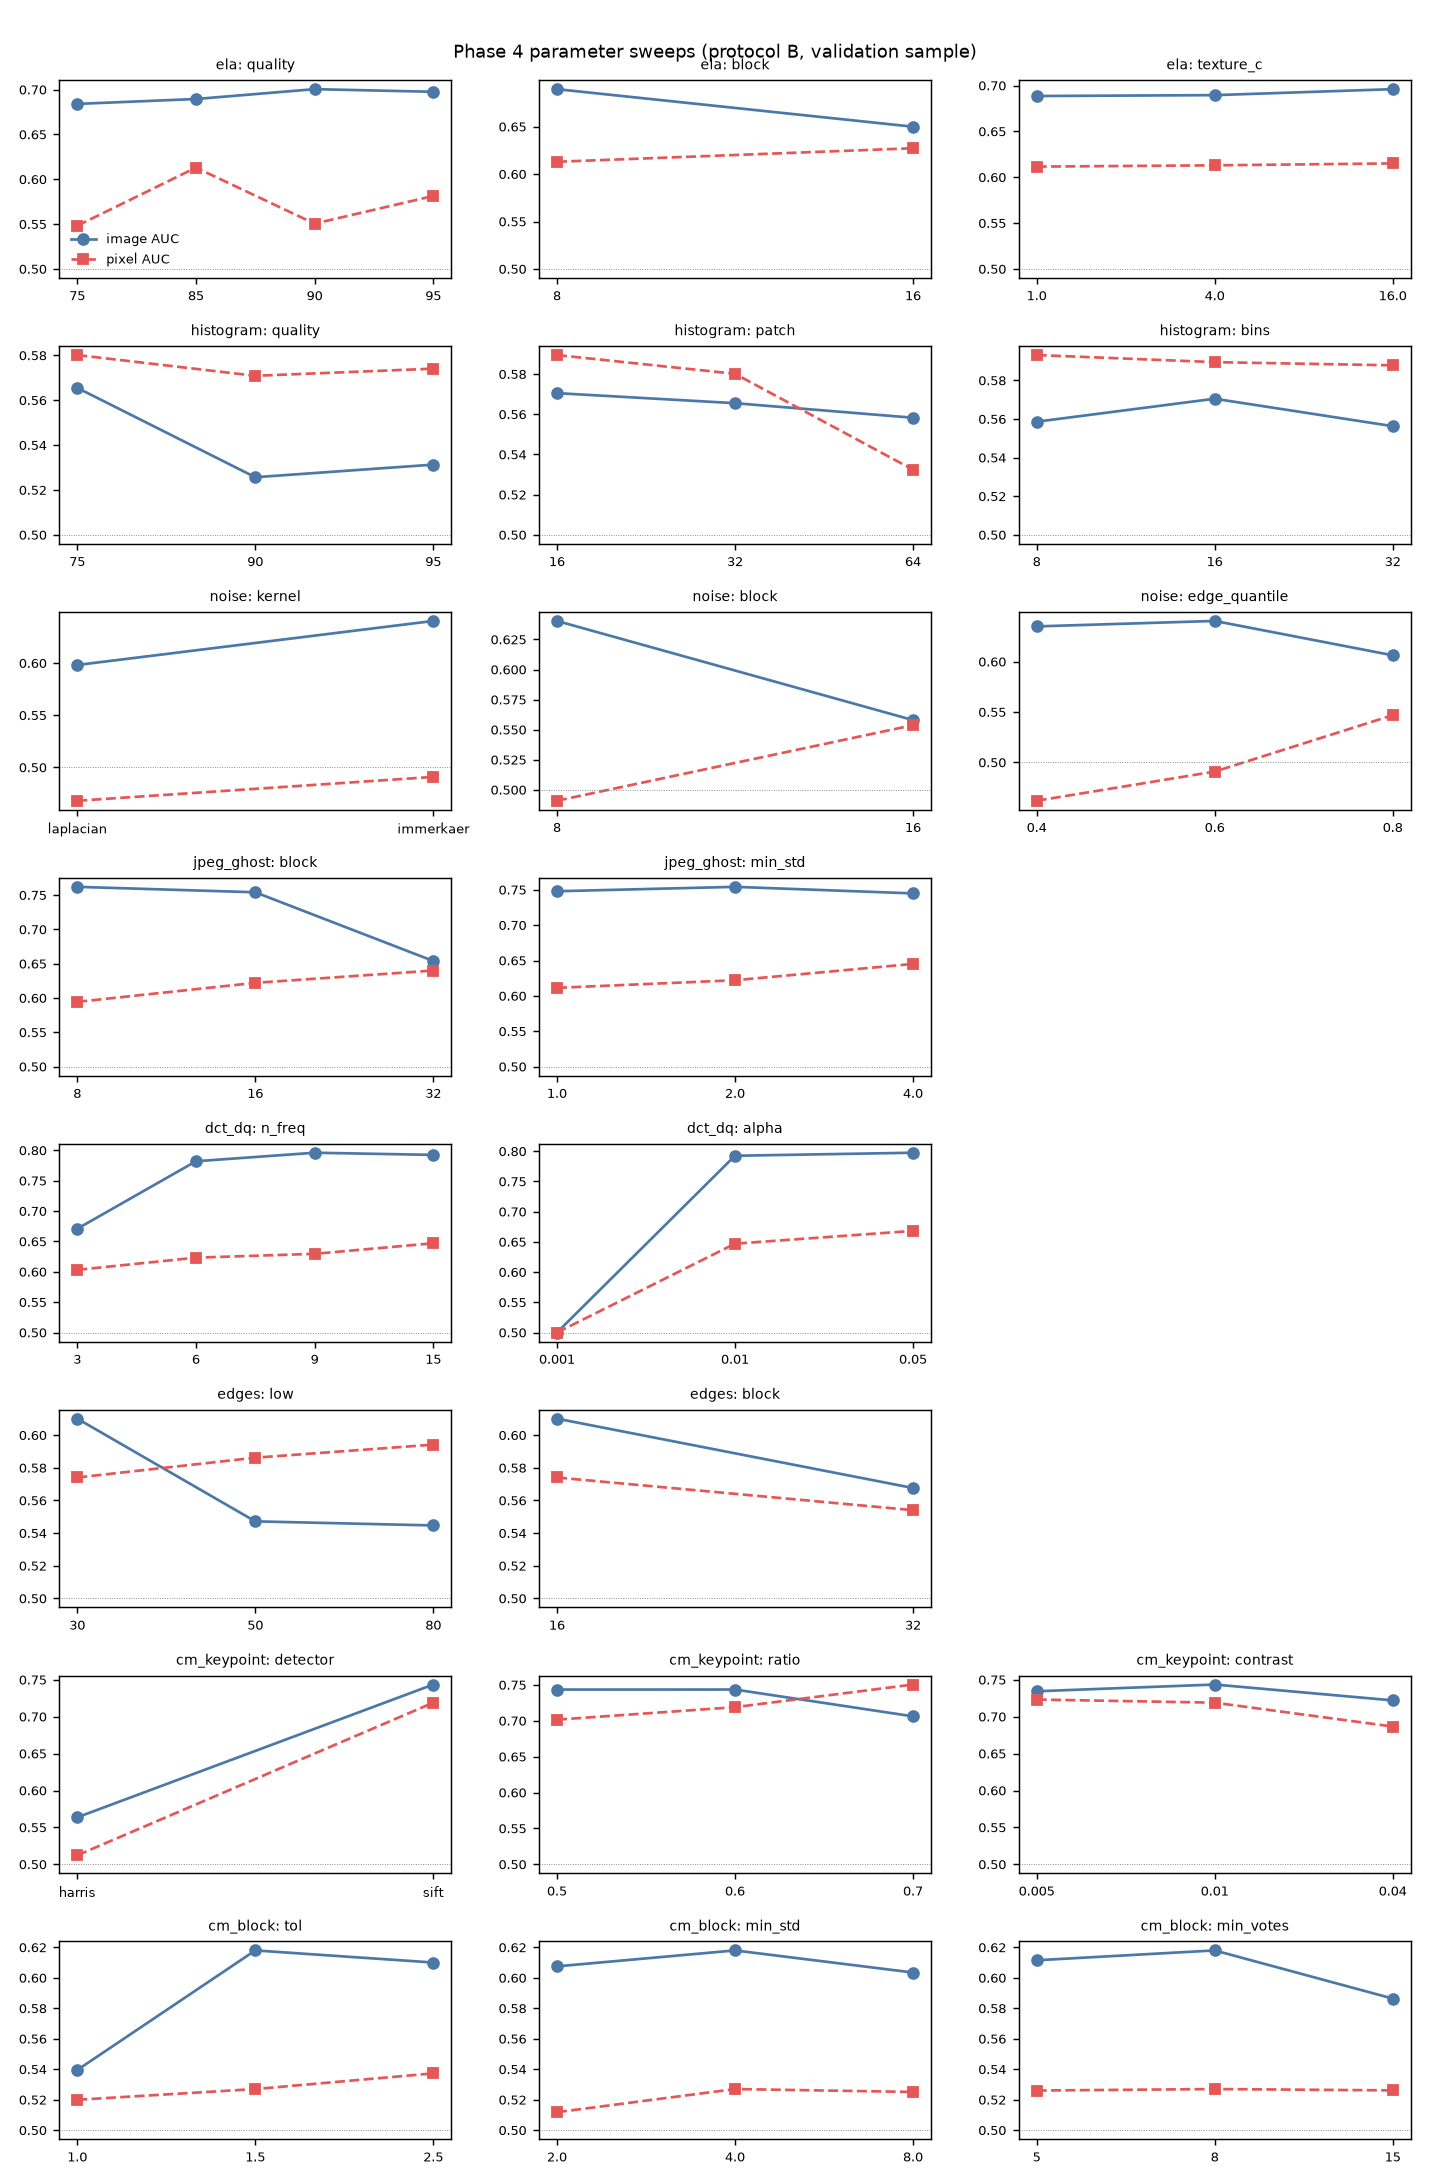
\includegraphics[width=\textwidth,height=0.84\textheight,keepaspectratio]{fig_sweeps.png}
\caption{Parameter sweeps under protocol B on the validation sample: image AUC (blue, circles) and pixel AUC (red,
squares) for each value of each swept parameter, one row per module.}
\label{fig:sweeps}
\end{figure}
}{}
\IfFileExists{sections/appendix_classification.tex}{\section{Classification: Full Results}\label{app:classification}
\begingroup\sloppy\urlstyle{tt}
Full results behind Section~\ref{sec:classification} (script \texttt{scripts/run\_phase5.py}). Table~\ref{tab:app-cls-auc} repeats Table~\ref{tab:cls-auc} with fold standard deviations; all protocols were re-run after the corrections to the feature modules described in Section~\ref{sec:method}. The ablations and the copy-move study (Tables~\ref{tab:app-ablation} and~\ref{tab:app-copymove}) use the most frequently selected hyper-parameters rather than nested selection, so they are mildly optimistic.

\begin{table}[!ht]
\centering
\caption{Out-of-fold ROC-AUC, mean $\pm$ std over 5 folds.}
\label{tab:app-cls-auc}
\footnotesize
\begin{tabular}{lccccc}
\toprule
Features & B: RF & B: SVM & R: RF & R: SVM & A: RF \\
\midrule
Shortcuts (Section~\ref{sec:leakage}) & 0.876 $\pm$ 0.003 & 0.876 $\pm$ 0.010 & 0.721 $\pm$ 0.013 & 0.771 $\pm$ 0.010 & \textbf{1.000} \\
Forensic, local only & 0.902 $\pm$ 0.003 & -- & \textbf{0.781 $\pm$ 0.012} & -- & 0.962 \\
Forensic, local + global & 0.910 $\pm$ 0.003 & 0.892 $\pm$ 0.004 & \textbf{0.795 $\pm$ 0.008} & 0.793 $\pm$ 0.006 & 0.978 \\
Forensic + shortcuts & 0.926 $\pm$ 0.004 & 0.922 $\pm$ 0.004 & 0.810 $\pm$ 0.006 & \textbf{0.826 $\pm$ 0.008} & 0.999 \\
\bottomrule
\end{tabular}
\end{table}

\begin{table}[!ht]
\centering
\caption{Module ablations (RF, fixed hyper-parameters): ROC-AUC of each module alone, and AUC lost when it is removed from the full forensic set.}
\label{tab:app-ablation}
\footnotesize
\begin{tabular}{lcccc}
\toprule
Module & Alone, B & Alone, R & Lost if removed, B & Lost if removed, R \\
\midrule
ELA & 0.723 & 0.664 & $-$0.000 & \textbf{0.013} \\
Patch-histogram $\chi^2$ & 0.569 & 0.566 & $-$0.001 & $-$0.001 \\
Noise level & 0.645 & 0.617 & $-$0.000 & 0.004 \\
JPEG ghosts & 0.758 & 0.624 & 0.010 & 0.001 \\
DCT double quantisation & \textbf{0.821} & 0.519 & \textbf{0.046} & 0.001 \\
Edge sharpness & 0.626 & 0.605 & $-$0.001 & 0.002 \\
Copy-move keypoints & 0.747 & \textbf{0.720} & \textbf{0.039} & \textbf{0.080} \\
Copy-move blocks & 0.600 & 0.579 & 0.000 & 0.003 \\
\bottomrule
\end{tabular}
\end{table}

\begin{table}[!ht]
\centering
\caption{Copy-move detectors compared (copy-move vs authentic images; pixel-level figures from Section~\ref{sec:params}).}
\label{tab:app-copymove}
\footnotesize
\begin{tabular}{lcccc}
\toprule
 & Image AUC, B & Image AUC, R & Pixel AUC, B & Share localised (pixel AUC $>$ 0.6), B \\
\midrule
Keypoints (SIFT + mirror) & 0.865 & 0.821 & 0.719 & 56\% \\
Blocks (DCT + mirror) & 0.633 & 0.603 & 0.527 & 14\% \\
Both & 0.878 & 0.839 & -- & -- \\
\bottomrule
\end{tabular}
\end{table}

Among the copy-move detectors (Table~\ref{tab:app-copymove}), keypoint matching dominates, but block matching still adds a little (0.865 $\to$ 0.878 under B, 0.821 $\to$ 0.839 under R); presumably it catches some copies in regions where few keypoints are found (not verified). Block matching also votes above threshold on some authentic images (32\% of 25 authentic training images in a check made before the module was corrected), which is one reason it is weak on its own.

\begin{table}[!ht]
\centering
\caption{Chosen ``uncertain'' band per protocol (smallest band reaching 85\% accuracy while judging at least half of the images).}
\label{tab:app-band}
\footnotesize
\begin{tabular}{lcccc}
\toprule
Protocol & Uncertain band & Share judged & Accuracy on judged & Balanced accuracy on judged \\
\midrule
R & $P(\text{tampered}) \in 0.5 \pm 0.24$ & 51\% & 0.855 & 0.810 \\
B & $P(\text{tampered}) \in 0.5 \pm 0.04$ & 96\% & 0.851 & 0.839 \\
\bottomrule
\end{tabular}
\end{table}

Table~\ref{tab:app-band} lists the uncertain band chosen for each protocol (Section~\ref{sec:classification-calib}). The deployed models are trained on all dev images and stored as \url{models/forgery_{B,R}.joblib} and \url{models/type_{B,R}.joblib}; \texttt{models/MAIN\_PROTOCOL} = R, so \texttt{detect.py} uses protocol R by default. Running \texttt{detect.py} on train or val images therefore gives in-sample outputs that look much better than reality.

\paragraph{Sources of optimism} The nested-CV numbers of Tables~\ref{tab:cls-auc} and~\ref{tab:cls-added} select hyper-parameters inside each training fold. The other analyses are mildly optimistic: the ablations, the copy-move study, calibration, the uncertain band, SHAP and the final models use the hyper-parameters selected most often across the five outer folds, a choice made by looking at all folds; the feature-module parameters were tuned (Section~\ref{sec:params}) on 3,400 dev images (2,400 train + 1,000 val) that also lie inside the CV folds; the band is chosen on the same out-of-fold predictions it is evaluated on; and SHAP is computed in-sample. The deployed model of each protocol is trained on all dev images with that protocol's most frequently selected hyper-parameters, isotonic calibration and its own uncertain band. Only the test-set evaluation (Section~\ref{sec:test}) is free of all of these.

Fig.~\ref{fig:calibration} shows the calibration and accuracy--coverage curves behind Section~\ref{sec:classification-calib}.

\begin{figure}[!ht]
\centering
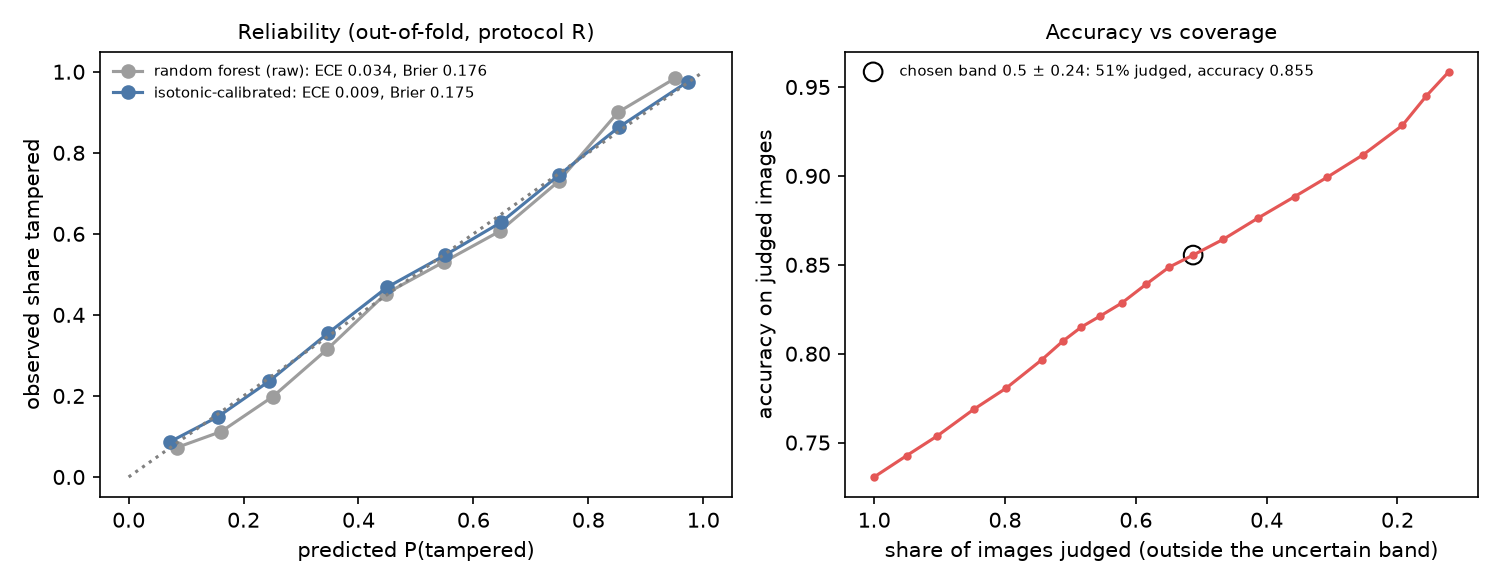
\includegraphics[width=0.85\textwidth]{fig_calibration_R.png}
\caption{Protocol R, out-of-fold. Left: reliability diagram of the raw and isotonic-calibrated random forest. Right: accuracy on judged images versus the share of images judged as the uncertain band widens; the circle marks the chosen band $0.5 \pm 0.24$.}
\label{fig:calibration}
\end{figure}
\par\endgroup
}{}
\IfFileExists{sections/appendix_localisation.tex}{\section{Localisation: Additional Details}\label{app:localisation}
\begingroup\sloppy\urlstyle{tt}
Details behind Section~\ref{sec:localisation}. The fusion code is in \url{src/forgery/localize/fusion.py}; the scripts are \url{scripts/extract_maps.py}, \url{scripts/run_phase6.py} and \url{scripts/phase6_gating.py}.

\paragraph{Training cells and post-processing grid} The learned fusions are trained on cells of training images: every tampered training image with a valid mask, plus 1,000 authentic training images. Up to 400 tampered and 400 untampered cells are sampled per image, about 2.1--2.3 million cells in all. The post-processing grid is $t \in 0.05\ldots0.95$; opening $\in \{1, 5, 9\}$; closing $\in \{1, 9, 17\}$; minimum area $\in \{0, 0.2\%, 1\%\}$. The threshold is chosen first, without morphology; the morphology settings are then chosen at that threshold. The margins between the learned fusions are small, so selecting the main method on the same numbers matters little.

\paragraph{Confidence intervals} 95\% group-bootstrap CIs for the gradient-boosted fusion (Table~\ref{tab:loc-methods}): under R, F1\ci{0.168}{0.200}, IoU\ci{0.108}{0.130}, MCC\ci{0.140}{0.176}; under B, F1\ci{0.237}{0.282}, IoU\ci{0.160}{0.193}, MCC\ci{0.230}{0.277}. The threshold-free pixel ROC-AUC is computed on every second pixel. The oracle F1 uses the best threshold per image without morphology; post-processing beats it on some images, so it is not a strict upper bound.

\begin{table}[!ht]
\centering
\caption{Gradient-boosted fusion by tampered area (validation).}
\label{tab:app-loc-area}
\footnotesize
\begin{tabular}{lccc}
\toprule
Tampered area & F1, R & Pixel AUC, R & F1, B \\
\midrule
$<$ 1\% & 0.034 & 0.617 & 0.10 \\
1--5\% & 0.162 & 0.736 & 0.27 \\
$>$ 5\% & 0.309 & 0.706 & 0.35 \\
\bottomrule
\end{tabular}
\end{table}

Table~\ref{tab:app-loc-area} gives the per-area breakdown: very small regions are essentially not localised, although their pixel AUC is still above chance.

\paragraph{Gating} On authentic images the fused mask is rarely empty: under R, with the final (deployed) post-processing, gradient boosting marks some region on 89\% of authentic validation images, with a mean area of 5.6\%; the out-of-sample figures are almost the same (88.8\%, 5.7\%). The system therefore shows the mask only when the calibrated image-level verdict is not ``authentic''. For evaluation, the out-of-fold forest scores of the validation images are mapped through the deployed model's isotonic calibrator and gated with the deployed band. This approximates fully out-of-fold calibrated scores; the calibrator itself was fitted on grouped out-of-fold scores of the whole dev set, validation included. Table~\ref{tab:loc-gating} shows that gating removes a large share of false regions at a small cost in tampered-image F1, because images judged authentic by mistake lose their mask. The gated F1 values use the final post-processing, tuned on all validation images, so they are slightly optimistic compared with Table~\ref{tab:loc-methods}.

\begin{table}[!ht]
\centering
\caption{Effect of gating on validation images (ungated $\to$ gated).}
\label{tab:loc-gating}
\footnotesize
\begin{tabular}{lcccc}
\toprule
 & Authentic & Mean false & Tampered & Tampered \\
 & with a region & area & shown & F1 \\
\midrule
R ($\pm$0.24) & 89\% $\to$ \textbf{42\%} & 5.6\% $\to$ 3.7\% & 84\% & 0.186 $\to$ 0.175 \\
B ($\pm$0.04) & 71\% $\to$ \textbf{10\%} & 2.5\% $\to$ 0.7\% & 76\% & 0.261 $\to$ 0.225 \\
\bottomrule
\end{tabular}
\end{table}

\paragraph{Deployed localiser} \texttt{models/localizer\_\{R,B\}.joblib} holds the gradient-boosting fusion (trained on training cells) and the post-processing tuned on all validation images: R, $t = 0.60$, no opening, no closing, minimum area 0.2\%; B, $t = 0.70$, no opening, closing 17, minimum area 0.2\%. \texttt{detect.py} writes \texttt{mask.png} and \texttt{overlay.png} next to \texttt{report.json}. The localiser reuses the evidence maps that \texttt{detect()} already computes, so localisation adds almost no run time. Tampered images without a valid mask (19 in the whole dataset, 1 of them in the validation set) are excluded from localisation scoring.

\begin{figure}[!ht]
\centering
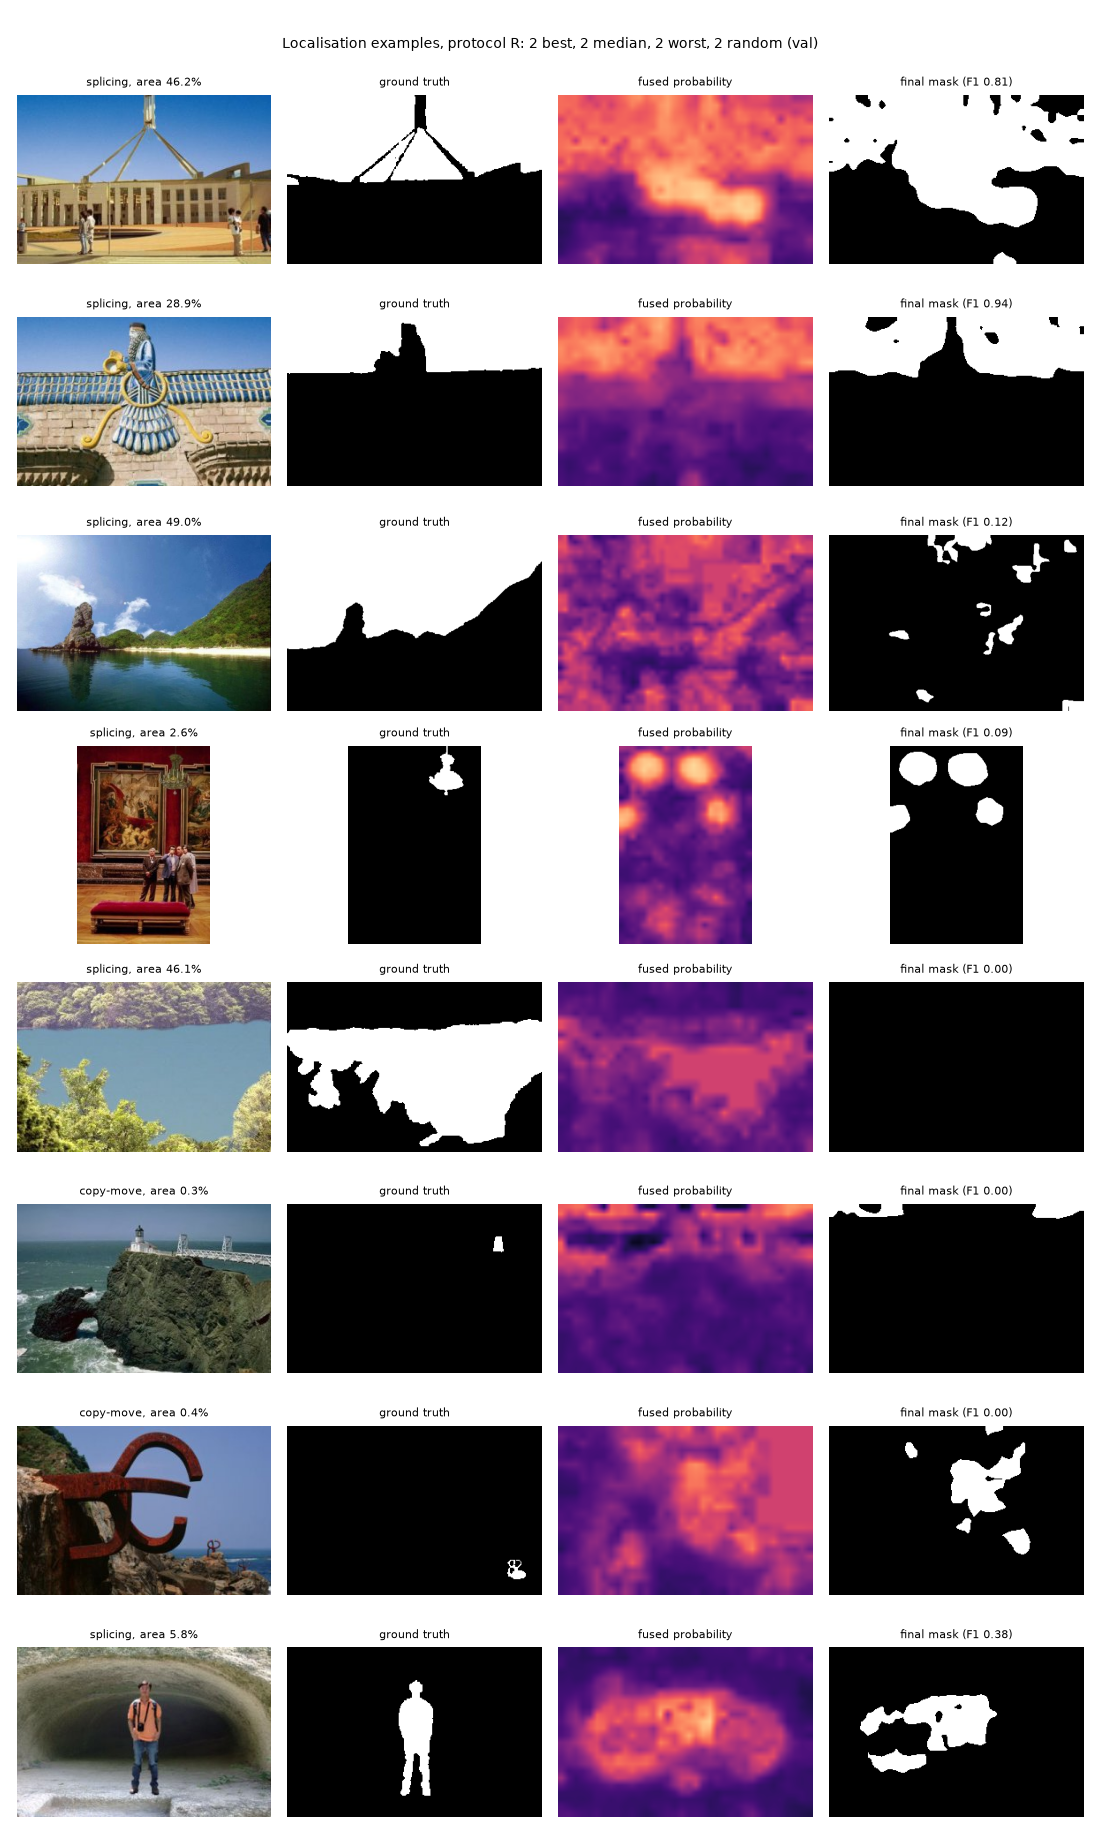
\includegraphics[width=0.6\textwidth]{fig_loc_examples_R.png}
\caption{Localisation examples under protocol R (validation): two best, two median, two worst and two random images. Columns: image with forgery type and tampered area, ground-truth mask, fused gradient-boosting probability, and final mask with its pixel F1. Failure modes visible here: tiny regions, where the probability peak lands elsewhere; large uniform pasted areas (sky, water); and textured authentic regions that attract spurious evidence.}
\label{fig:loc-examples}
\end{figure}
\par\endgroup
}{}
\IfFileExists{sections/appendix_test.tex}{\section{Test-Run Audit Trail}\label{app:test}
This appendix details the safeguards of the one-time test evaluation summarised in Section~\ref{sec:test}
(script \texttt{scripts/run\_phase7.py}; post-hoc analysis of the saved outputs in
\texttt{scripts/phase7\_posthoc.py}; outputs in \texttt{results/phase7/run\_1/}).
\begin{itemize}\setlength\itemsep{0pt}
\item \emph{Frozen models.} The classifiers were refit on all development images with the hyper-parameters
selected most often in the nested cross-validation; the refit of the main forensic random forest is identical to
the deployed model's forest. The deployed calibrated models were used with their uncertain bands, and the deployed
localisers with their post-processing. Localisation baselines had their post-processing tuned on the validation
images only.
\item \emph{Dry runs.} Before the test run, the full script was exercised twice in a dry-run mode, with the
training images as ``development'' and the validation images as ``test''. It was then checked in an independent code review.
\item \emph{Preflight.} At run time a preflight confirmed that every model, feature file and cache matched the
current code and configuration.
\item \emph{Start record.} The start record in \texttt{results/phase7/test\_runs.log} holds fingerprints of 36
files (all project source files and \texttt{config.yaml}) and of 12 input files (the frozen split's hash file,
the models and the classification and localisation inputs they were built from).
\item \emph{Completion record.} Because of a path bug, run~1 wrote its completion record, with the hashes of
\texttt{summary.json} and \texttt{test\_classification.csv}, into \texttt{run\_1/test\_runs.log}. The record was
copied, unchanged and annotated, into the main log after the run, and the bug was then fixed. The fix changes the
script's fingerprint for any future run.
\item \emph{Output manifest.} A SHA-1 manifest of every output file of run~1 (\texttt{run\_1/MANIFEST.sha1}) was
recorded on the same day.
\item \emph{Post-run check.} A post-run check recomputed the code and input fingerprints and found nothing
changed since the run started.
\end{itemize}
The later uses of the test split, namely the post-hoc robustness, synthetic and external evaluations with the same
frozen models (Section~\ref{sec:robustness}) and the pre-registered, one-time comparison with an ELA-CNN baseline
(Section~\ref{sec:cnn}; new models, evaluated once), fed nothing back and are recorded in the same log
(Appendix~\ref{app:repro}).
}{}
\IfFileExists{sections/appendix_robustness.tex}{\section{Robustness Experiments: Details}\label{app:robustness}
These details complement Section~\ref{sec:robustness} (script \texttt{scripts/run\_phase7b.py}; outputs in
\texttt{results/phase7b/}: \texttt{robustness.csv}, \texttt{synthetic.csv}, \texttt{external.csv},
\texttt{summary.json}, \texttt{micc\_paired\_R\_minus\_B.json}).

\textbf{Degradations.} JPEG re-compression at qualities 95, 85, 75, 65 and 50; downscaling by $\times$0.9,
$\times$0.75 and $\times$0.5, with the ground-truth mask resized alongside; Gaussian blur with $\sigma=0.5$, 1.0
and 1.5; Gaussian noise with $\sigma=2$, 5 and 10 grey levels; and a simulated social-media upload ($\times$0.8
downscale, then JPEG quality 70). Each degradation was applied before the protocol (R or B). Fig.~\ref{fig:robustness}
plots every condition.

\begin{figure}[h]
\centering
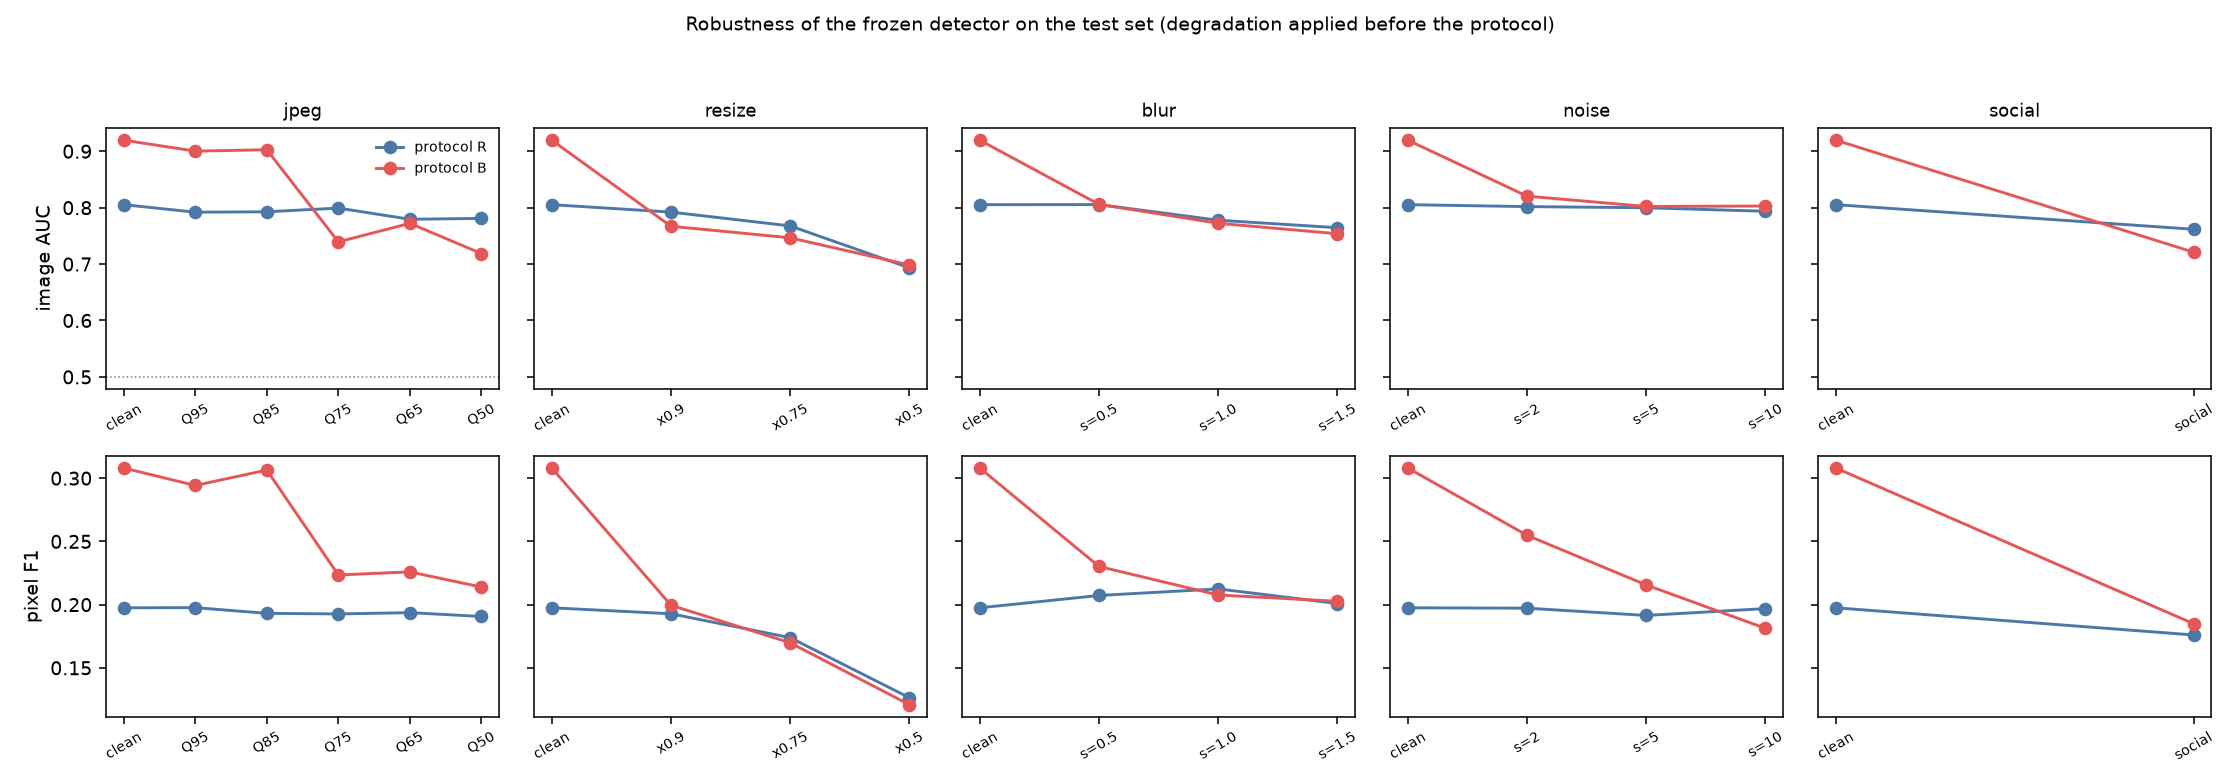
\includegraphics[width=\textwidth]{fig_robustness.png}
\caption{Robustness of the frozen detector on the test set, degradation applied before the protocol. Top: image
AUC; bottom: pixel F1; columns: JPEG quality, downscaling, Gaussian blur, Gaussian noise and a simulated
social-media upload. Protocol R (blue) stays nearly flat except under strong downscaling; protocol B (red) loses
its advantage after re-compression below Q85 and under blur, noise or downscaling.}
\label{fig:robustness}
\end{figure}


\textbf{Synthetic mask definitions.} Hard-splice and copy-move masks are exact: no pixel outside the mask changes.
Poisson blending also alters pixels around the pasted region, so a seamless splice's mask is the pasted region
plus every pixel the blending changed by more than 2 grey levels. For copy-moves the mask is the pasted copy; we
also score copy-move localisation against source $\cup$ copy, because the localiser marks both. In 112 of 240
copy-moves the copy partly overlaps and hides the source (in 34 by more than 20\,\%).

\textbf{Manual forgeries.} Forgeries made by hand in an image editor, and real messaging-app round trips, were not
available. The synthetic set is a controlled stand-in, and adding real hand-made examples is left as optional
further work.

\textbf{External datasets not tested.} COVERAGE~\cite{wen2016coverage} (hosted behind an authenticated OneDrive
link), the Columbia splicing set (server refused access) and CASIA v1.0 (account needed) could not be downloaded
automatically. Of the MICC datasets, F600, the version with masks, was offline, and F2000 (4\,GB) was skipped. A
cross-dataset splicing test is therefore missing.
}{}
\IfFileExists{sections/appendix_cnn.tex}{\section{ELA-CNN: Training Details and Additional Results}\label{app:cnn}

\textbf{Selection and training.} The network was trained on the train split (8,828 images) with horizontal flips,
class-weighted binary cross-entropy, AdamW (learning rate $3\cdot10^{-4}$, weight decay $10^{-4}$), batch 64 and a
cosine schedule over at most 15 epochs; the epoch and pooling rule were selected by AUC on the validation split (1,894
images). Early stopping ended training after 4 epochs without improvement in validation AUC;
nothing besides the epoch and the pooling rule was tuned, because a second 5-fold CV, as used for the classical models,
would have cost about $15\times20$~min of GPU time. Table~\ref{tab:app-cnn-sel} lists the selected recipes and
Fig.~\ref{fig:app-cnn-training} the validation curves. Training and refitting took about 3.5~hours on an Apple M4 GPU
(MPS backend), which is not bit-reproducible. A preflight step checked the models, the ELA settings, the classical
scores and every cached comparison result before the single test run, whose start and completion are recorded in the
run log. Code: \texttt{scripts/make\_ela.py}, \texttt{scripts/run\_phase8.py}, \texttt{scripts/phase8\_posthoc.py} and
\texttt{src/forgery/cnn.py}.

\textbf{ELA input.} Fig.~\ref{fig:cnn-ela} shows the network's input for two validation images, as released and after
protocol R. The authentic JPEG shows almost no ELA error as released, while the tampered TIFF shows strong error along
edges and texture: the format leak is visible in ELA itself.

\begin{figure}[!ht]
\centering
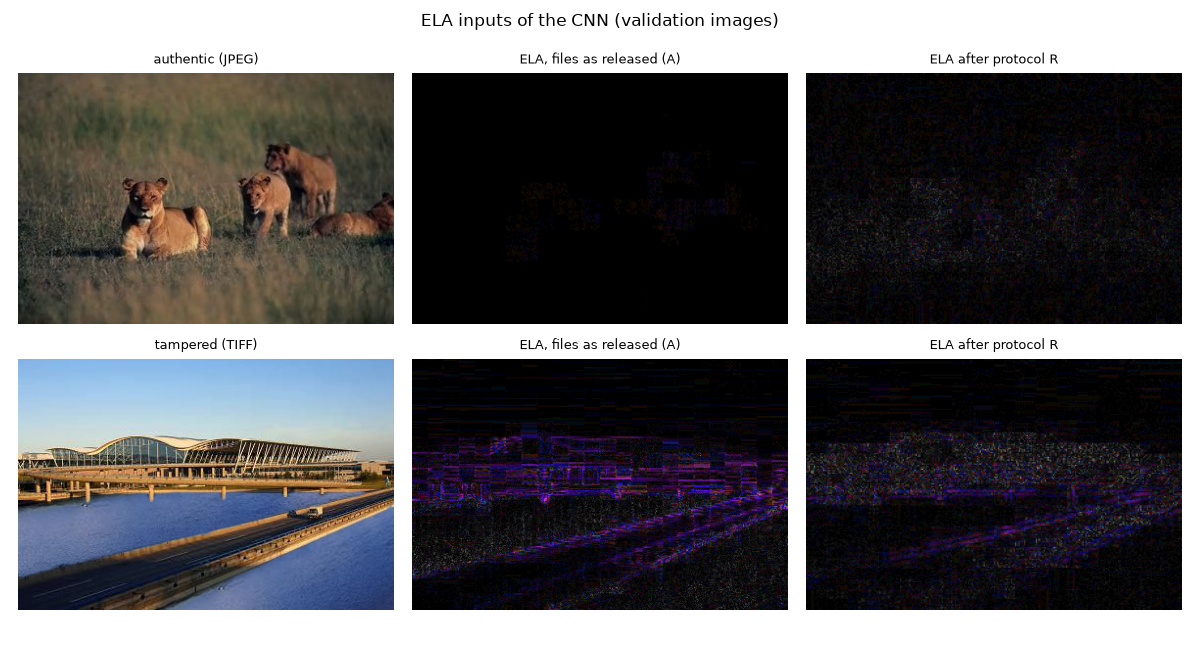
\includegraphics[width=0.7\textwidth]{fig_ela_examples.png}
\caption{ELA inputs of the CNN for two validation images. Top: an authentic JPEG, whose ELA as released (A) is almost
black. Bottom: a tampered TIFF, whose ELA as released shows strong error along edges and texture. Right: ELA of the
same images after protocol R.}
\label{fig:cnn-ela}
\end{figure}


\begin{table}[!ht]
\centering
\caption{Selected epoch and pooling rule per protocol (train split; validation split for selection).}
\label{tab:app-cnn-sel}
\footnotesize
\begin{tabular}{lccl}
\toprule
Protocol & Selected epoch & Pooling & Validation AUC \\
\midrule
R & 3 & max & 0.746 (seeds 42 / 43 / 44: 0.746 / 0.762 / 0.752) \\
B & 8 & mean & 0.797 \\
A & 12 & mean & 0.994 \\
\bottomrule
\end{tabular}
\end{table}

\begin{figure}[!ht]
\centering
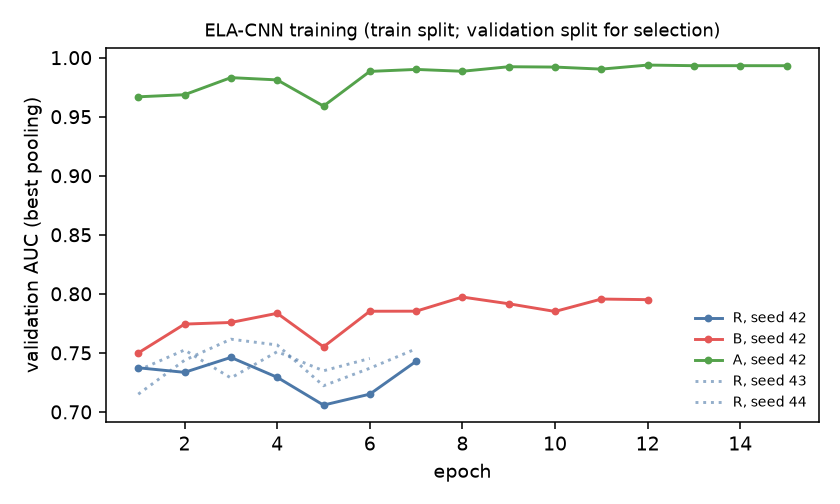
\includegraphics[width=0.6\textwidth]{fig_cnn_training.png}
\caption{Validation AUC (best pooling) per epoch of the ELA-CNN under A, B and R; under R for three seeds.}
\label{fig:app-cnn-training}
\end{figure}

\textbf{Image size.} Table~\ref{tab:app-cnn-size} extends the post-hoc size grouping of Section~\ref{sec:cnn-groups}.
The train-only selection models show the same drop on validation: R 0.728 on standard-size vs.\ 0.567 on larger
images; B 0.792 vs.\ 0.664. Under B, larger authentic images also receive higher scores than standard-size authentic
ones (mean logit 0.17 vs.\ $-$1.76). Within the larger images, the score correlates only weakly with the number of
tiles (Spearman 0.20 under R, max pooling; $-$0.09 under B, mean pooling). Against the forest on forensic + shortcut
features, the CNN differs by $-$0.045\ci{$-$0.074}{$-$0.017} (R), $-$0.125\ci{$-$0.145}{$-$0.104} (B) and
$-$0.005\ci{$-$0.009}{$-$0.003} (A). Under B, CNN $-$ classical is $-$0.129\ci{$-$0.152}{$-$0.106} on copy-move and
$-$0.071\ci{$-$0.101}{$-$0.042} on splicing.

\begin{table}[!ht]
\centering
\caption{Test AUC by natural image size (post-hoc; the pre-registered area terciles are invalid).}
\label{tab:app-cnn-size}
\footnotesize
\begin{tabular}{lcccccc}
\toprule
Size (test images) & $n$ & Tampered & R: CNN & R: classical & R: CNN $-$ classical & B: CNN $-$ classical \\
\midrule
Smaller than $384\times256$ & 21 & 62\% & 0.702 & 0.615 & +0.087\ci{$-$0.072}{0.260} & $-$0.144 \\
$384\times256$, either orientation & 1,469 & 34\% & 0.770 & 0.789 & $-$0.019\ci{$-$0.065}{0.026} & $-$0.105\ci{$-$0.133}{$-$0.080} \\
Larger than $384\times256$ & 402 & 65\% & 0.544 & 0.730 & $-$0.186\ci{$-$0.232}{$-$0.139} & $-$0.217\ci{$-$0.266}{$-$0.163} \\
\bottomrule
\end{tabular}
\end{table}

\textbf{Robustness.} Table~\ref{tab:app-cnn-robust} gives the test AUC after each degradation of
Section~\ref{sec:robustness}; each was followed by the protocol and then ELA (classical results are the frozen outputs
of that section). Under R, the CNN loses about as much as the classical pipeline: JPEG Q75 costs 0.008 vs.\ 0.006,
resize $\times$0.5 0.085 vs.\ 0.112, and the social upload 0.037 vs.\ 0.044; after resizing, the gap between the two
is not significant ($-$0.008\ci{$-$0.043}{0.027}). Under B, the classical pipeline loses much more, because its B
advantage rests on compression traces that any re-save overwrites: JPEG Q75 costs it 0.180 against 0.065 for the CNN,
leaving the two level (+0.007\ci{$-$0.034}{0.047}), and the social upload 0.199 against 0.137. Padding is not the cause of
the CNN's losses: after downscaling most images become smaller than one tile (95\% under R resize $\times$0.5; 82\%
after a social upload), and scoring them without padding changes the AUC by at most 0.018. On MICC-F220 the CNN reaches
0.529\ci{0.360}{0.700} (R) and 0.454\ci{0.226}{0.660} (B), consistent with chance, while the classical detector
reaches 0.972 (R) and 0.902 (B); the CIs are wide because the forgeries come from only 11 scenes. The failure fits the
size analysis: all MICC-F220 photographs are larger than CASIA's standard size ($722\times480$ to $800\times1{,}070$)
and come from a different dataset, whereas the classical copy-move matching finds the duplicated regions regardless of
their source.

\begin{table}[!ht]
\centering
\caption{Test AUC of the ELA-CNN and the classical pipeline under degradations and on MICC-F220.}
\label{tab:app-cnn-robust}
\footnotesize
\begin{tabular}{lccccc}
\toprule
Condition & R: CNN & R: classical & R: rank average & B: CNN & B: classical \\
\midrule
clean & 0.770 & 0.805 & 0.824 & 0.811 & 0.920 \\
JPEG Q75 & 0.762 & 0.799 & 0.817 & 0.746 & 0.739 \\
resize $\times$0.5 & 0.685 & 0.693 & 0.720 & 0.672 & 0.698 \\
social upload & 0.733 & 0.762 & 0.788 & 0.674 & 0.721 \\
MICC-F220 & 0.529\ci{0.360}{0.700} & 0.972 & 0.811 & 0.454\ci{0.226}{0.660} & 0.902 \\
\bottomrule
\end{tabular}
\end{table}
}{}
\IfFileExists{sections/appendix_system.tex}{\section{System: Implementation, Tests and Limitations}\label{app:system}

\textbf{Code.} \texttt{src/forgery/pipeline.py} (\texttt{detect()}), \texttt{src/forgery/explain.py} (explanations,
input preparation and reports; no interface code), \texttt{detect.py} (command line) and \texttt{app/} (Streamlit
interface, started with \texttt{streamlit run app/Home.py}). The PDF report holds the verdict, overlay, evidence chart
and caveats on the first page and the eight evidence maps on the second. The command-line tool and both analysis pages
use the same input preparation. The detector's loader converts every image with PIL's \texttt{convert("RGB")}; this
is correct for CASIA, where all 12,614 images are 8-bit RGB without EXIF rotation, but it would turn a 16-bit greyscale
image white. A changed image is saved losslessly as PNG; under B and R the detector works on decoded pixels, so this
does not affect the analysis. The explorer shows only the 10,722 training and validation images, and since the
deployed models were refit on all development images, their results on CASIA examples are optimistic.

\textbf{Input preparation.} Every user image is fully decoded, so truncated files fail early; decompression bombs and
images outside 64--4,000~px per side are refused; the image is rotated by its EXIF orientation, and 16-bit or float
images are rescaled to 8~bits.

\textbf{Performance.} Table~\ref{tab:sys-perf} gives run times on an Apple M4 laptop. Models are loaded once and
cached.

\begin{table}[!ht]
\centering
\caption{Run time on an Apple M4 laptop (largest allowed image: $4{,}000\times2{,}667$~px).}
\label{tab:sys-perf}
\footnotesize
\begin{tabular}{lcc}
\toprule
Step & CASIA-sized & Largest (R / B) \\
\midrule
Detection, all eight modules & $\approx$0.2~s & 4.3~s / 7.1~s \\
SHAP explanation & $\approx$0.5~s & $\approx$0.5~s \\
PDF report & $\approx$0.3~s & 2.0~s / 3.3~s \\
\bottomrule
\end{tabular}
\end{table}

\textbf{Interface details.} The analysis page accepts JPEG, PNG, TIFF, BMP and WebP (at most 4,000~px per side) and, for
CASIA examples, also shows the ground truth. The batch page shows a progress bar, a table of verdicts, probabilities,
region sizes and the strongest evidence, a gallery of images judged tampered, and CSV and ZIP (overlay) downloads. The
dataset explorer shows ground-truth masks and metadata (format, estimated JPEG quality, IJG tables, tampered area,
host and donor id, split group). The results dashboard covers leakage, classification, localisation, the test set,
robustness and MICC-F220, and the CNN comparison; it shows saved figures made from test images (the missed forgeries
and false alarms of Section~\ref{sec:test} and the synthetic forgeries of Section~\ref{sec:robustness}), which are
outputs of the one-time evaluation, not a way to browse the test set. Uploads are stored once per content hash, so a
rerun (a protocol switch back or a download click) reuses the cached analysis and PDF, also for rotated or 16-bit
photos, whose prepared copy is written once; batch results are kept in the session until the input or the protocol
changes; stored uploads are deleted after seven days.

\textbf{Tests.} \texttt{tests/test\_app.py} runs every page headlessly with Streamlit's AppTest framework and checks
that no page raises an exception; the analysis page produces a verdict for an example image; the batch page processes
a folder containing a corrupt file and reports exactly that file as an error; a batch in which every file fails still
renders and hidden files are skipped; batch results survive a rerun; and an empty explorer filter does not blank the
other tabs. \texttt{tests/test\_explain.py} checks that 16-bit images are rescaled, not clipped; EXIF rotation is
applied; truncated, non-image, too-small and too-large files are refused; and ordinary files pass through unchanged.
All pages were also exercised in headless Chrome, including a batch run and the example analysis; the screenshots come
from that run.

\textbf{Limitations.} (i)~Local use only: nothing is uploaded to a server, but the folder mode reads any folder the user
names, so the configuration binds the server to \texttt{localhost}. (ii)~An EXIF-rotated photo is analysed upright;
several modules work on fixed block grids, so the same photo rotated by 90$^\circ$ can receive a different score.
(iii)~The suspected region is shown for uncertain images too, for inspection, matching the command-line tool, which
removes the region only for images judged authentic.
}{}


\end{document}
